\chapter{Teoría de Aproximaciones: Bases Reducidas y Aprendizaje}


En la primera sección de este capítulo se dará una introducción al enfoque de bases reducidas, un método de aproximación fundamental en el modelado de orden reducido \cite{Tiglio:2021ysj}. 
%Este marco tiene dos etapas bien diferenciadas; por un lado la parte de entrenamiento, que puede ser bastante costosa pero que solo debe realizarse una vez, y después la parte de evaluación, que es mucho más rápida y puede utilizarse múltiples veces.
Luego, en la segunda sección se ampliará con el refinamiento hp \textit{greedy} \cite{Cerino:2022dhr}; una metodología que descompone de forma iterativa el dominio de parámetros para crear bases reducidas locales de forma adaptativa.

%\section{Aproximación por Proyección}
%Antes de entender las bases reducidas es necesario tener claro como se aproxima un vector o función a un dado espacio.
%Sea $W_n \mathcal{W}_n$ un espacio vectorial n-dimensional y subespacio de un espacio de Hilbert $\mathcal{H}$

\section{Bases Reducidas}

El objetivo de este método es obtener una base que represente un espacio de soluciones de forma aproximada pero con alta precisión, evitando tener que resolver el problema completo múltiples veces para generar más soluciones. 
%En este contexto las soluciones son ondas gravitacionales y resolver el problema consistiría en tener que obtener soluciones costosas utilizando relatividad numérica.

Las bases reducidas son un método de expansión espectral, así como la expansión de Fourier o los polinomios de Jacobi. La diferencia de este método es que los elementos de la base serán soluciones del espacio que se quiere aproximar (no necesariamente funciones trigonométricas o polinomios, como en lo otros métodos mencionados).

Para la construcción de una base reducida se parte de un espacio de soluciones \mbox{$\mathcal{F}:= \{ h_{\lambda} = h_{\lambda}(t) = h(\lambda, t)\}$}, donde $h_{\lambda}$ representa una onda gravitacional parametrizada por $\lambda \in \Omega$, siendo $\Omega$ un dominio compacto de parámetros (cada parámetro $\lambda$ es multidimensional y representa los parámetros mencionados anteriormente, como la relación entre masas o los espines de los agujeros negros).

Se realiza un muestreo de $\mathcal{F}$ y $\Omega$ para construir un conjunto de entrenamiento $\mathcal{T} := \{\lambda_i, h_{\lambda_i}\}_{i=1}^N$ con $N$ elementos. A partir de este conjunto $\mathcal{T}$, se construye una base $\{e_i\}_{i=1}^n$, generalmente con $n << N$, de forma que se pueda generar el conjunto $\{h_{\lambda_i}\}_i^N$, e incluso el espacio $\mathcal{F}$, con la combinación lineal:

%Para construir la base se parte de un conjunto de entrenamiento $\mathcal{T} := \{\lambda_i, h_{\lambda_i}\}_{i=1}^N$, resultado de un muestreo $\mathcal{K} := \{h_{\lambda_i}\}_{i=1}^n$de $\mathcal{F}$, y que contiene la información del conjunto de parámetros $\{\lambda_i\}_{i=1}^n$ utilizado para la construcción de cada función de $\mathcal{K}$. A partir de $\mathcal{T}$ se construye una base $\{e_i\}_{i=1}^n$, generalmente con $n << N$. Luego se puede representar $\mathcal{K}$, e incluso $\mathcal{F}$ con la combinación lineal

\begin{equation}
\label{eq:rb0}
h_{\lambda} (t) \approx \sum_{i=1}^{n} c_{i,\lambda} e_i(t).
\end{equation}

Luego utilizando un conjunto de validación se puede obtener una medida del error o precisión con la que dicha base representa al espacio original.

\subsection{Elección de una base óptima}

%Antes de poder representar $\mathcal{F}$ se necesita encontrar una base óptima dado un error de tolerancia $\varepsilon$ y/o un máximo número de elementos en la base $n_{max}$.
La pregunta de que tan bien se puede aproximar el espacio $\mathcal{F}$ a partir de una base $\{e_i\}_{i=1}^n$ se puede caracterizar utilizando la definición de la distancia de Kolmogorov \cite{Pinkus1985nWidthsIA}:

\begin{equation} \label{eq:kolmogorov}
d_n := \min_{\{e_i\}_{i=1}^n} \max_{\lambda \in \Omega} \min_{ c_{i,\lambda} \in \mathbb{C}} \| h_{\lambda} - \sum_{i=1}^{n} c_{i,\lambda} e_i(t)\|^2.
\end{equation}



Esta distancia es básicamente es una medida del máximo error de representación en un espacio compacto de parámetros $\Omega$, con una base y coeficientes óptimos.

El producto interno $\|\cdot\|$ en \eqref{eq:kolmogorov} está dado por

\[
\|h_{\lambda}\|^2 :=\int_{t_i}^{t_f}|h_{\lambda}(t)|^2dt
\]
definido a partir del producto interno
\[
\langle h_1, h_2 \rangle  :=\int_{t_i}^{t_f} \overline{h_{1}}(t) h_2 (t)dt
\]

Para entender la notación en $d_n$, se explica el signifcado de los $\min$, $\max$, $\min$ de derecha a izquierda:

\begin{itemize}
\item $\min_{ c_{i,\lambda} \in \mathbb{C}}$ se refiere a la representación óptima con respecto a la base utilizada. Esto implica realizar una proyección ortogonal a la base. Suponiendo una base ortonormal los coeficientes óptimos serán:

\begin{equation} \label{eq:coefs}
c_{i, \lambda} = \langle e_i, h_{\lambda} \rangle 
\end{equation}

Y se puede reescribir la ecuación \eqref{eq:kolmogorov} de la siguiente forma:
\[
d_n := \min_{\{e_i\}_{i=1}^n} \max_{\lambda \in \Omega} || h_{\lambda} - \mathcal{P}_nh_{\lambda} ||^2.
\]

con 
\begin{equation}
\mathcal{P}_nh_{\lambda} = \sum_{i=1}^{n} c_{i,\lambda} e_i(t)
\end{equation}

\item $\max_{\lambda \in \Omega}$ hace referencia a que se tiene en cuenta el peor error (el máximo) en el espacio de parámetros $\Omega$. 
\item Por último $\min_{\{e_i\}_{i=1}^n}$ implica elegir la base óptima que de lugar al \textit{mejor peor error} en el dominio de parámetros.
\end{itemize}

Por lo tanto $d_n$ sirve como un límite superior; es lo mejor que se puede lograr si la base fue escogida de forma óptima.
En algunos casos $d_n$ se puede calcular teóricamente \cite{MAGARILILYAEV200197}. Más específicamente se puede probar que $d_n \sim n^{-r}$ para funciones con sus primeras $(r-1)$ derivadas continuas y que $d_n \sim e^{-an^b}$ para funciones con una dependencia $C^{\infty}$  \cite{articleg}. En el contexto de ondas gravitacionales se espera un comportamiento asíntotico de convergencia exponencial con $n$ \citep{PhysRevX.4.031006, Herrmann:2012xpx}.

La elección de una base óptima es una tarea complicada de complejidad combinatoria y no aplicable en la práctica. Por lo tanto se utilizará un acercamiento más eficiente en base al uso de un algoritmo de tipo voraz o \textit{greedy}, que da lugar a una base cuasi-óptima en un sentido matemático, de complejidad lineal. Para más detalles se recomienda ver \cite{Tiglio:2021ysj}.

\subsection{Algoritmo \textit{Greedy} para construir una base cuasi-óptima}

Un algoritmo de tipo \textit{greedy} es un proceso iterativo en el cual a cada paso se toma la elección que produzca el mayor beneficio inmediato.

En el contexto de las bases reducidas, cada iteración del algoritmo agregará a la base el elemento que daba lugar al peor (máximo) error de representación con la base anterior. Es decir que en cada iteración se reducirá el máximo error de representación de todo el conjunto de entrenamiento.

Para cada solución $h_{\lambda}$ del conjunto de entrenamiento, el error de representación es $\| h_{\lambda} - \mathcal{P}_nh_{\lambda} \|^2$, por lo tanto el máximo error de representación o ``Error \textit{greedy}", se define como :

\begin{equation}
\sigma_n := \max_{\lambda \in  \{ \lambda_{i}\}_{i=1}^N } \| h_{\lambda} - \mathcal{P}_nh_{\lambda} \|^2.
\end{equation}

Este error es el \textit{error de entrenamiento}, que disminuirá con cada iteración del algoritmo. También se hablará del \textit{error de validación}, que es el máximo error de representación que ocurre dentro de un conjunto de validación, generalmente más denso que el conjunto de entrenamiento.

El proceso de construcción de una base reducida se puede ver en el algoritmo \ref{alg:rb}, y se explica a continuación:

\begin{itemize}
\item Al algoritmo ingresan tres elementos:
	\begin{itemize}
	\item [--] Un conjunto de entrenamiento $\mathcal{T} = \{ \lambda_{i}, h(\lambda_i) \}_{i=1}^N$ (que incluye tanto las funciones de onda como los parámetros de las funciones), 
	\item[--] El número máximo de elementos permitidos en la base $n_{max}$,
	\item[--] El mínimo error de tolerancia $\varepsilon$ también llamado \textit{tolerancia greedy}.
	\end{itemize}

\item El primer elemento de la base reducida se elije de forma arbitraria a partir del conjunto de parámetros $\{\lambda_{i}\}_{i=1}^N$. El primer parámetro elegido se llama \textit{semilla} o primer parámetro \textit{greedy} $\Lambda_1$. Luego el primer elemento será $h(\Lambda_1)$, pero normalizado.
\item Luego iterativamente se agregan nuevos elementos a la base, seleccionando los parámetros que den lugar al mayor error dentro del conjunto de entrenamiento. El conjunto de estos parámetros recibe el nombre de \textit{parámetros greedy}.
\item Por conveniencia a la hora de realizar proyecciones en el espacio generado por la base, se construye una base ortonormal (de forma que los coeficientes $c_{i,\lambda}$ se obtengan por medio de la ecuación \eqref{eq:coefs}). Para esto se aplica un algoritmo de ortonormalización de Gram-Schmidt (líneas 9 y 10 del algoritmo \ref{alg:rb}).
\item El algoritmo finaliza cuando se alcanzó el número máximo de elementos en la base $n = n_{max}$, o cuando el máximo error de representación $\sigma_n$ sea menor al error de tolerancia $\varepsilon$, lo que ocurra primero. El algoritmo devuelve los elementos de la base reducida $\{ e_i\}_{i=1}^{n}$, el conjunto de parámetros \textit{greedy} $\{\Lambda_i\}_{i=1}^{n}$ y el error de representación $\sigma_n$.
\end{itemize}

\begin{algorithm}
\caption{\texttt{GreedyRB}\((\mathcal{T}, \varepsilon, n_{max})\)}\label{alg:rb}
\begin{algorithmic}[1]
\Require $\mathcal{T} = \{ \lambda_{i}, h(\lambda_i) \}_{i=1}^N, \varepsilon, n_{max}$ 
\vspace{3mm}
\State $i = 1$
\State $\sigma_1 = 1$ \Comment{Inicializar error de representación a 1}
\State $\Lambda_1 = \lambda_k$	\Comment{Elección arbitraria de la semilla}
\State $e_1 = h(\Lambda_1)/||h(\Lambda_1)||$	
\State $\text{rb}=\{e_1\}$	\Comment{Primer elemento de la base reducida}
\vspace{2mm}
\While{$\sigma_i > \varepsilon$ \textbf{and} $i < n_{max}$}
	\State $i = i+1$
	\State $\Lambda_i = 	arg \max_{\lambda \in \mathcal{T}}||h_{\lambda}-\mathcal{P}_{i-1}h_{\lambda}||^2$ \Comment{Selección del parámetro \textit{greedy}}
	\State $e_i = h(\Lambda_i) - {P}_{i-1}h(\Lambda_i)$ \Comment{Gram-Schmidt}
	\State $e_i = e_i / ||e_i|| $ \Comment{Normalización}	
	\State $\text{rb} = \text{rb} \cup \{e_i\}$
	\State $\sigma_i = \max_{\lambda \in \mathcal{T}}||h_{\lambda}-\mathcal{P}_{i}h_{\lambda}||^2$	\Comment{Error de representación}
\EndWhile
\vspace{3mm}
\Ensure $\text{rb} = \{ e_i\}_{i=1}^{n},\Lambda = \{\Lambda_i\}_{i=1}^{n}, \sigma_n$
\end{algorithmic}
\end{algorithm}


\subsection{Convergencia del Algoritmo \textit{Greedy}}

Para una tolerancia \textit{greedy} $\varepsilon$ el algoritmo \textit{greedy} entrega una base reducida con un error

\[
\sigma_n = \max_{\lambda \in  \{ \lambda_{i}\}_{i=1}^N } || h_{\lambda} - \mathcal{P}_nh_{\lambda} ||^2 \leq \varepsilon
\]

Dado que la elección del primer elemento de la base reducida es arbitrario (la elección de la semilla), el lector o lectora podría preguntarse que tan relevante es esta elección a la hora de condicionar la convergencia del error de representación $\sigma_n$.
Como se mencionó anteriormente, la medida de Kolmogorov $d_n$ puede utilizarse como cota superior. 
Resultados obtenidos en \cite{https://doi.org/10.48550/arxiv.1204.2290} muestran que si $d_n$ decae exponencialmente, $\sigma_n$ también lo hará:

\[
d_n \leq De^{-an^{\alpha}} \ \ \rightarrow \ \ \sigma_n \leq \sqrt{2D} \gamma^{-1} e^{-a_{\alpha}'n^{\alpha}},
\]
con $D$, $\alpha$, $a$ constantes positivas y $\gamma \in (0,1]$.
De forma similar, si el decaimiento de $d_n$ es polinomial, también lo será el decaimiento de $\sigma_n$:
\[
d_n \leq D n^{-\alpha} \ \ \rightarrow \ \ \sigma_n \leq D_{\alpha}'n^{-\alpha},
\]
con $D$, $\alpha > 0$ y $\gamma \in (0, 1]$.

En la figura \ref{fig:rb_vs_n} se puede ver el decaimiento exponencial del error de representación en función del número de elementos de la base reducida aplicado en el contexto de ondas gravitacionales \cite{Caudill_2012}. Lo más relevante es que se puee ver que este comportamiento no depende de la elección de la raíz; el área sombreada representa los extremos de todas las posibles semillas dentro del conjunto de entrenamiento.


\begin{figure}[h!]
\centering
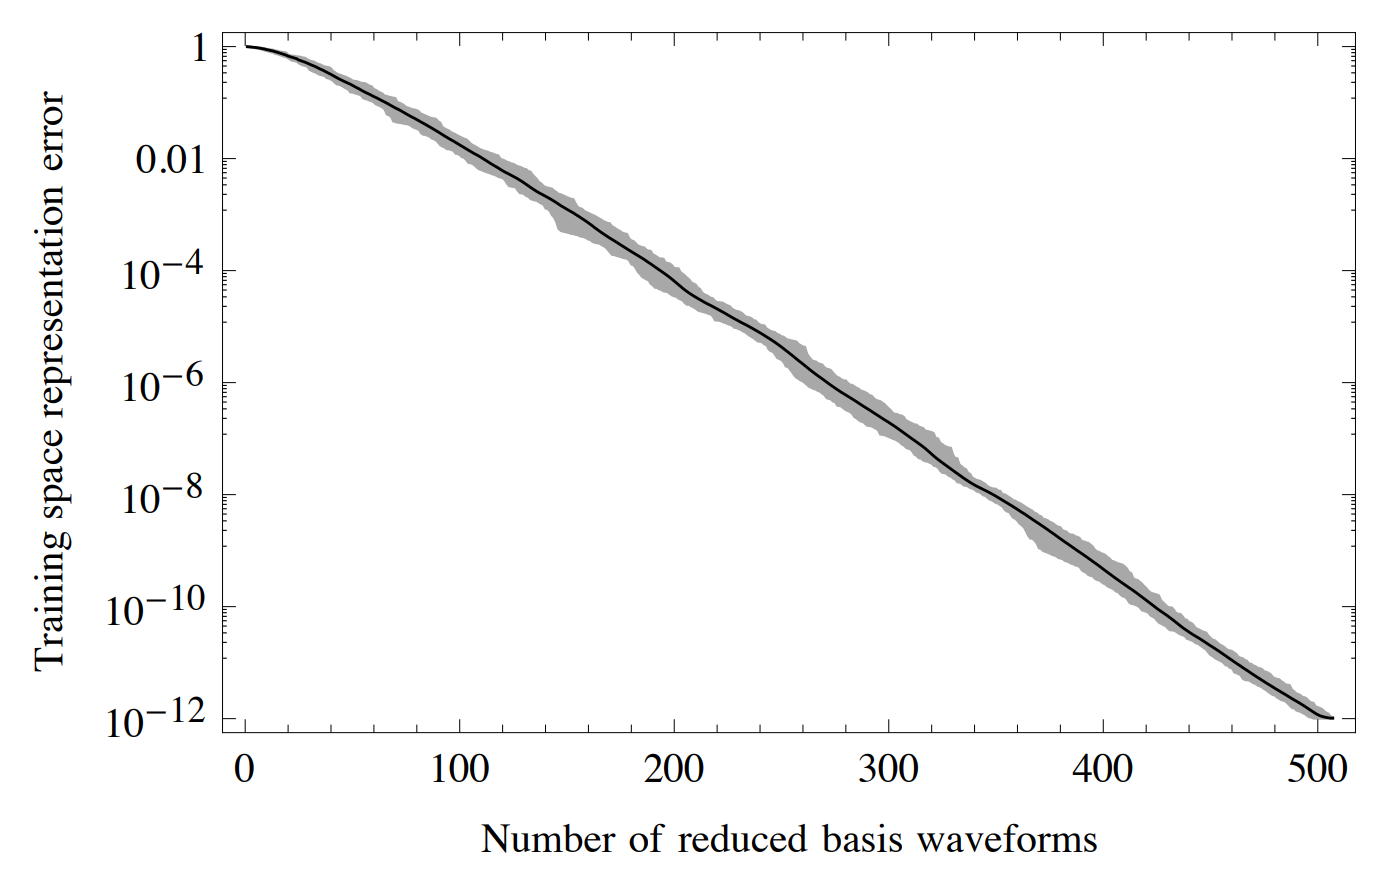
\includegraphics[width=.8\columnwidth]{figs/rb_vs_n.png}
\caption{Error de representación en función del número de funciones de onda en la base reducida para un modo cuasinormal (QNM). Se probaron todas las semillas posibles del conjunto de entrenamiento; en negrita se ve el promedio, y el área sombreada representa los valores extremos \cite{Caudill_2012}.}
\label{fig:rb_vs_n}
\end{figure}

\section{Bases Reducidas hp Greedy}

El nombre del método \textit{hp-greedy} \cite{Cerino:2022dhr} surge de la combinación del \textit{``refinamiento p''} y del \textit{``refinamiento h"}. El \textit{refinamiento p} proviene de los métodos espectrales con bases polinomiales \cite{hesthaven_gottlieb_gottlieb_2007} y se refiere a la propiedad de que el error de representación disminuye al aumentar el grado del polinomio (en el caso de las bases reducidas aumenta el número de elementos en la base). Por otro lado el término de \textit{refinamiento h} se toma prestado de los métodos de diferencias finitas, donde el tamaño de cada celda de la grilla es representado por \textit{h}, y este se refina para obtener un mejor resultado. En el caso de las bases reducidas \textit{hp-greedy} este último refinamiento ocurre en el espacio de los parámetros y no en el dominio físico.

\subsection{Refinamiento h}

Partiendo de la siguiente notación:
\begin{itemize}
\item $V$: espacio de parámetros para un dado subdominio.
\item $\Omega$: espacio total de parámetros tal que $\Omega= \cup V$.
\item $V_1, V_2$ : particiones de $V$.
\item $\Lambda_V$ : parámetros \textit{greedy} en $V$.
\item  $\hat{\Lambda}_{V}$: punto de anclaje para $V$.
%\item  $\hat{\Lambda}_{V_1}, \hat{\Lambda}_{V_2}$
\end{itemize}

El refinamiento en el dominio de los parámetros ocurre a partir de la división recursiva de cada subdominio $V \subseteq \Omega$ en dos subdominios $V_1$ y $V_2$. La división de cada dominio $V$ se realizará en función de dos puntos de anclaje $\hat{\Lambda}_{V_1}$ y $\hat{\Lambda}_{V_2}$. Estos puntos de anclaje no son más que los primeros dos elementos del conjunto de parámetros \textit{greedy} $\Lambda_V$.
Como resultado de estas divisiones iterativas se obtiene una estructura de árbol binario.


Esta descomposición binaria del dominio está descrita en forma de pseudocódigo en el algoritmo \ref{alg:part}.

Al algoritmo ingresan tres objetos:

\begin{itemize}
\item $\lambda_V$: conjunto de parámetros resultado de un muestreo de $V$.
\item $\hat{\Lambda}_{V_1}, \hat{\Lambda}_{V_2}$: puntos de anclaje (son los primeros dos elementos de $\Lambda_V$).
\end{itemize}

Luego, para cada parámetro del conjunto $\lambda_V$ se evalúa su distancia a los puntos de anclaje a partir de la \textit{función de proximidad} $d: d(\lambda_1, \lambda_2)$:

\[
d(\lambda_1, \lambda_2) = ||\lambda_1 - \lambda_2||_2,
\]

de forma que se obtengan dos conjuntos; $\lambda_{V_1}$ con los $\lambda_{i}$ más próximos a $\hat{\Lambda}_{V_1}$, y $\lambda_{V_2}$ con los $\lambda_{i}$ más próximos a $\hat{\Lambda}_{V_2}$, tal que  $\lambda_{V} =\lambda_{V_1} \cup \lambda_{V_2}$. Este resultado es la división del espacio de parámetros a partir de los puntos de anclaje.

\begin{algorithm}
\caption{\texttt{Partition}\((\lambda_V, \hat{\Lambda}_{V_1}, \hat{\Lambda}_{V_2})\)}\label{alg:part}
\begin{algorithmic}[1]
\Require $\lambda_V, \hat{\Lambda}_{V_1}, \hat{\Lambda}_{V_2}$ 
\vspace{3mm}
\State $\lambda_{V_1} = \lambda_{V_2} = \emptyset$
\For{\textbf{each} $\lambda_i \in \lambda_V$}
	\If{$d(\lambda_i, \hat{\Lambda}_{V_1}) <d(\lambda_i, \hat{\Lambda}_{V_2})$}
		\State $\lambda_{V_1} = \lambda_{V_1} \cup \lambda_i$
	\ElsIf{$d(\lambda_i, \hat{\Lambda}_{V_1}) >d(\lambda_i, \hat{\Lambda}_{V_2})$}
		\State $\lambda_{V_2} = \lambda_{V_2} \cup \lambda_i$
	\Else
		\State $\lambda_{V'} = $ random choice$([\lambda_{V_1}, \lambda_{V_2}])$
		\State $\lambda_{V'} = \lambda_{V'} \cup \lambda_i$
	\EndIf
\EndFor
\vspace{3mm}
\Ensure $\lambda_{V_1}, \lambda_{V_2}$
\end{algorithmic}
\end{algorithm}

\subsection{Refinamiento hp-greedy}


El refinamiento \textit{hp-greedy} es un método que combina el algoritmo greedy para la construcción de bases reducidas con la partición del dominio de parámetros. 

Esta partición recursiva del dominio de parámetros da lugar a una estructura de árbol binario, la cual tendrá diferentes niveles $l$ de profundidad, con un $l_{max}$ establecido por el usuario, de forma que $l : 0 \le l \le l_{max}$, donde $l =0$ es el nodo raíz. Cada nodo del árbol estará etiquetado por un conjunto de índices $B_l$, que parte de:

\[
B_0 = (0,),
\]
luego sus dos hijos ($l=1$) tendrán las etiquetas:
\[
B_1 = (0,0,) \ \ o \ \  (0, 1, ),
\]
y en general:
\[
B_l = (0, i_1, \cdots, i_l), \ \  con \ \ i_j = \{0, 1\},
\]

\noindent donde cada nivel $l$ tendrá un máximo de $2^l$ nodos.
Los nodos que no tengan hijos se llamarán nodos \textit{hojas}.
\begin{figure}[h!]
\centering
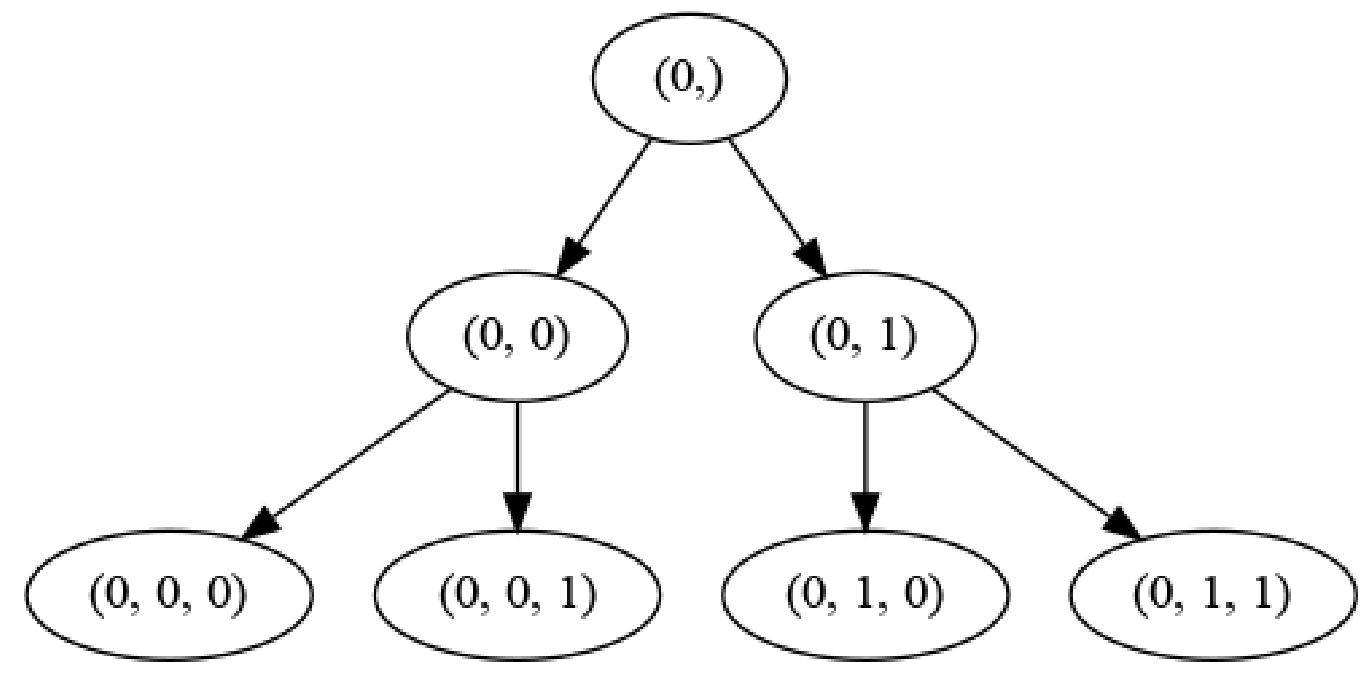
\includegraphics[width=.5\columnwidth]{Bl_lmax2.png}
\caption{Representación de los nodos de un árbol con $l_{max}=2$ \cite{Cerino:2022dhr}.}
\end{figure}

El método está explicado en el algoritmo \ref{alg:hp}; partiendo de un dado dominio de parámetros $V$ se construye una base reducida a partir de un conjunto de entrenamiento $\mathcal{T}_V = \{\lambda_{V_i}, h_{\lambda_{V_i}}\}_{i=1}^{N}$, una \textit{tolerancia greedy} $\varepsilon$ y un $n_{max}$ (para esto se utiliza el algoritmo \ref{alg:rb}). Si el error de representación $\sigma$ es mayor que la tolerancia $\varepsilon$, y si la profundidad del nivel $l$ es menor a $l_{max}$, entonces se realizará una partición del dominio $V$ utilizando como puntos de anclaje a los dos primeros parámetros \textit{greedy}. En cada dominio se realizará el mismo procedimiento hasta que se cumpla que $l = l_{max}$ o hasta que $\sigma \le \varepsilon$.

 % El conjunto $\lambda_V$ representa el conjunto de parámetros de $\mathcal{T}_V$

\begin{algorithm}
\caption{\texttt{hpGreedy}\((\mathcal{T}, \varepsilon, n_{max}, l, l_{max}, B_{l})\)}\label{alg:hp}
\begin{algorithmic}[1]
\Require $\mathcal{T} = \{ \lambda_{i}, h_{i} \}_{i=0}^N, \varepsilon, n_{max},l, l_{max}, B_{l}$ 
\vspace{3mm}
\State rb, $\Lambda_V$, $\sigma$ = \texttt{GreedyRB}($\mathcal{T}_V,\lambda_V, \varepsilon, n_{max}$) 
\vspace{3mm}
\If{$\sigma > \varepsilon$ \textbf{and} $l<l_{max}$}
	\State $\hat{\Lambda}_{V_1} = \Lambda_V[1]$
	\State $\hat{\Lambda}_{V_2} = \Lambda_V[2]$
	\State $\lambda_{V_1}, \lambda_{V_2} =$ \texttt{Partition}$(\lambda_V,\hat{\Lambda}_{V_1}, \hat{\Lambda}_{V_2})$
	\State $out_1 = $ \texttt{hpGreedy}\((\mathcal{T}_{V_1}, \lambda_{V_1}, \varepsilon, n_{max}, l+1, l_{max}, (B_{l}, 0))\)
	\State $out_2 = $ \texttt{hpGreedy}\((\mathcal{T}_{V_2} ,\lambda_{V_2}, \varepsilon, n_{max}, l+1, l_{max}, (B_{l}, 1))\)
	\State $out = out_1 \cup out_2$
\Else
	\State $out = \{( rb, \Lambda_V, B_l)\}$
\EndIf
\vspace{3mm}
\Ensure out
\end{algorithmic}
\end{algorithm}

El resultado del algoritmo \ref{alg:hp} es una estructura arbórea, donde cada nodo contiene la información de sus puntos de anclaje, por lo que en el caso de querer proyectar un conjunto de validación, cada onda gravitacional se proyectará a la base reducida del nodo hoja con el punto de anclaje más cercano al parámetro de la onda. En la figura \ref{fig:part_1d} se puede ver un esquema de la división de parámetros para el caso de un $\lambda$ de una sola dimensión. Luego en la figura \ref{fig:proy_1d} se esquematiza el proceso de proyección de una función $h_{\lambda_i}$ a la base creada.

\begin{figure}[h!]
\centering
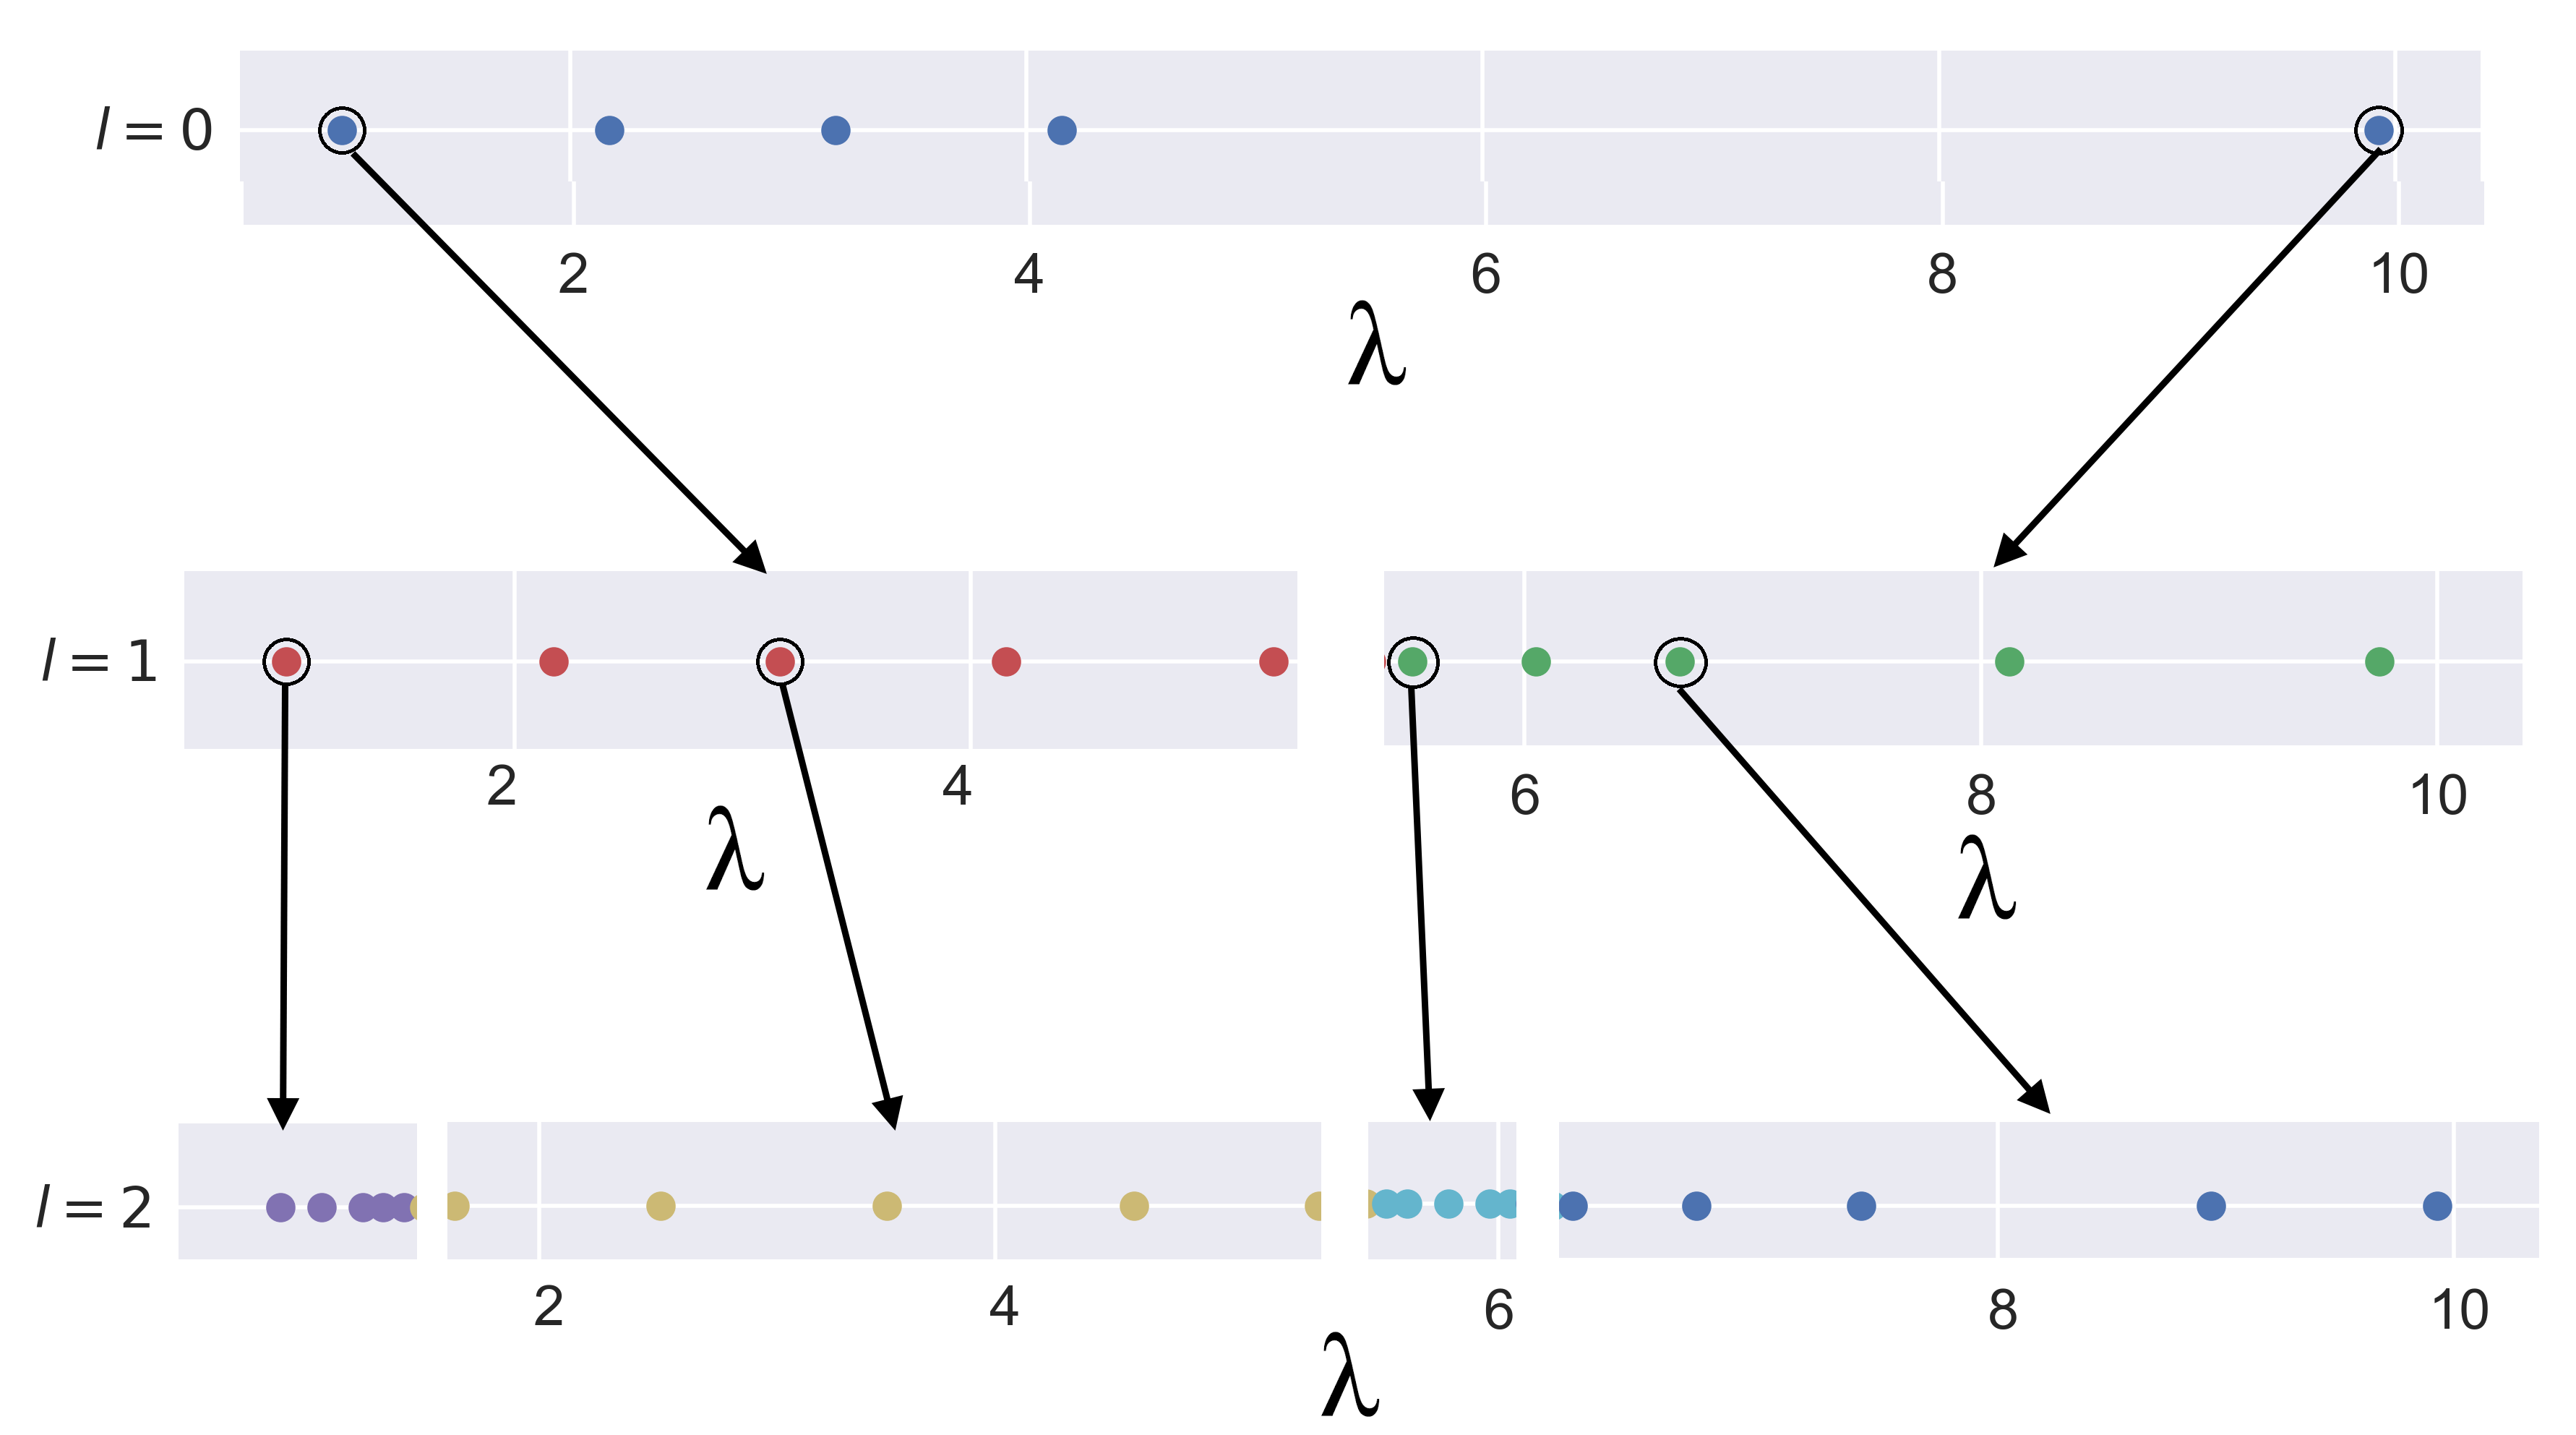
\includegraphics[width=0.75\columnwidth]{figs/particion_parametros_1d.png}
\caption{Ejemplo de partición del dominio de parametros para un parámetro $\lambda$ unidimensional. Los puntos de colores representan a los parámetros \textit{greedy} $\Lambda_V$ para cada subdominio $V$, resaltando a los puntos de anclaje $\Lambda_V$ con un círculo externo. Este diagrama muestra como se divide cada subdominio en función de sus puntos de anclaje. En este ejemplo $n_{max} = 5$ y $l_{max}=2$.}
\label{fig:part_1d}
\end{figure}

\subsection{Tiempo de Proyección}


Un aspecto muy importante del refinamiento \textit{hp-greedy}, que se mencionará seguido de ahora en adelante, es el tiempo de proyección a la base. 


\begin{figure}[h!]
\centering
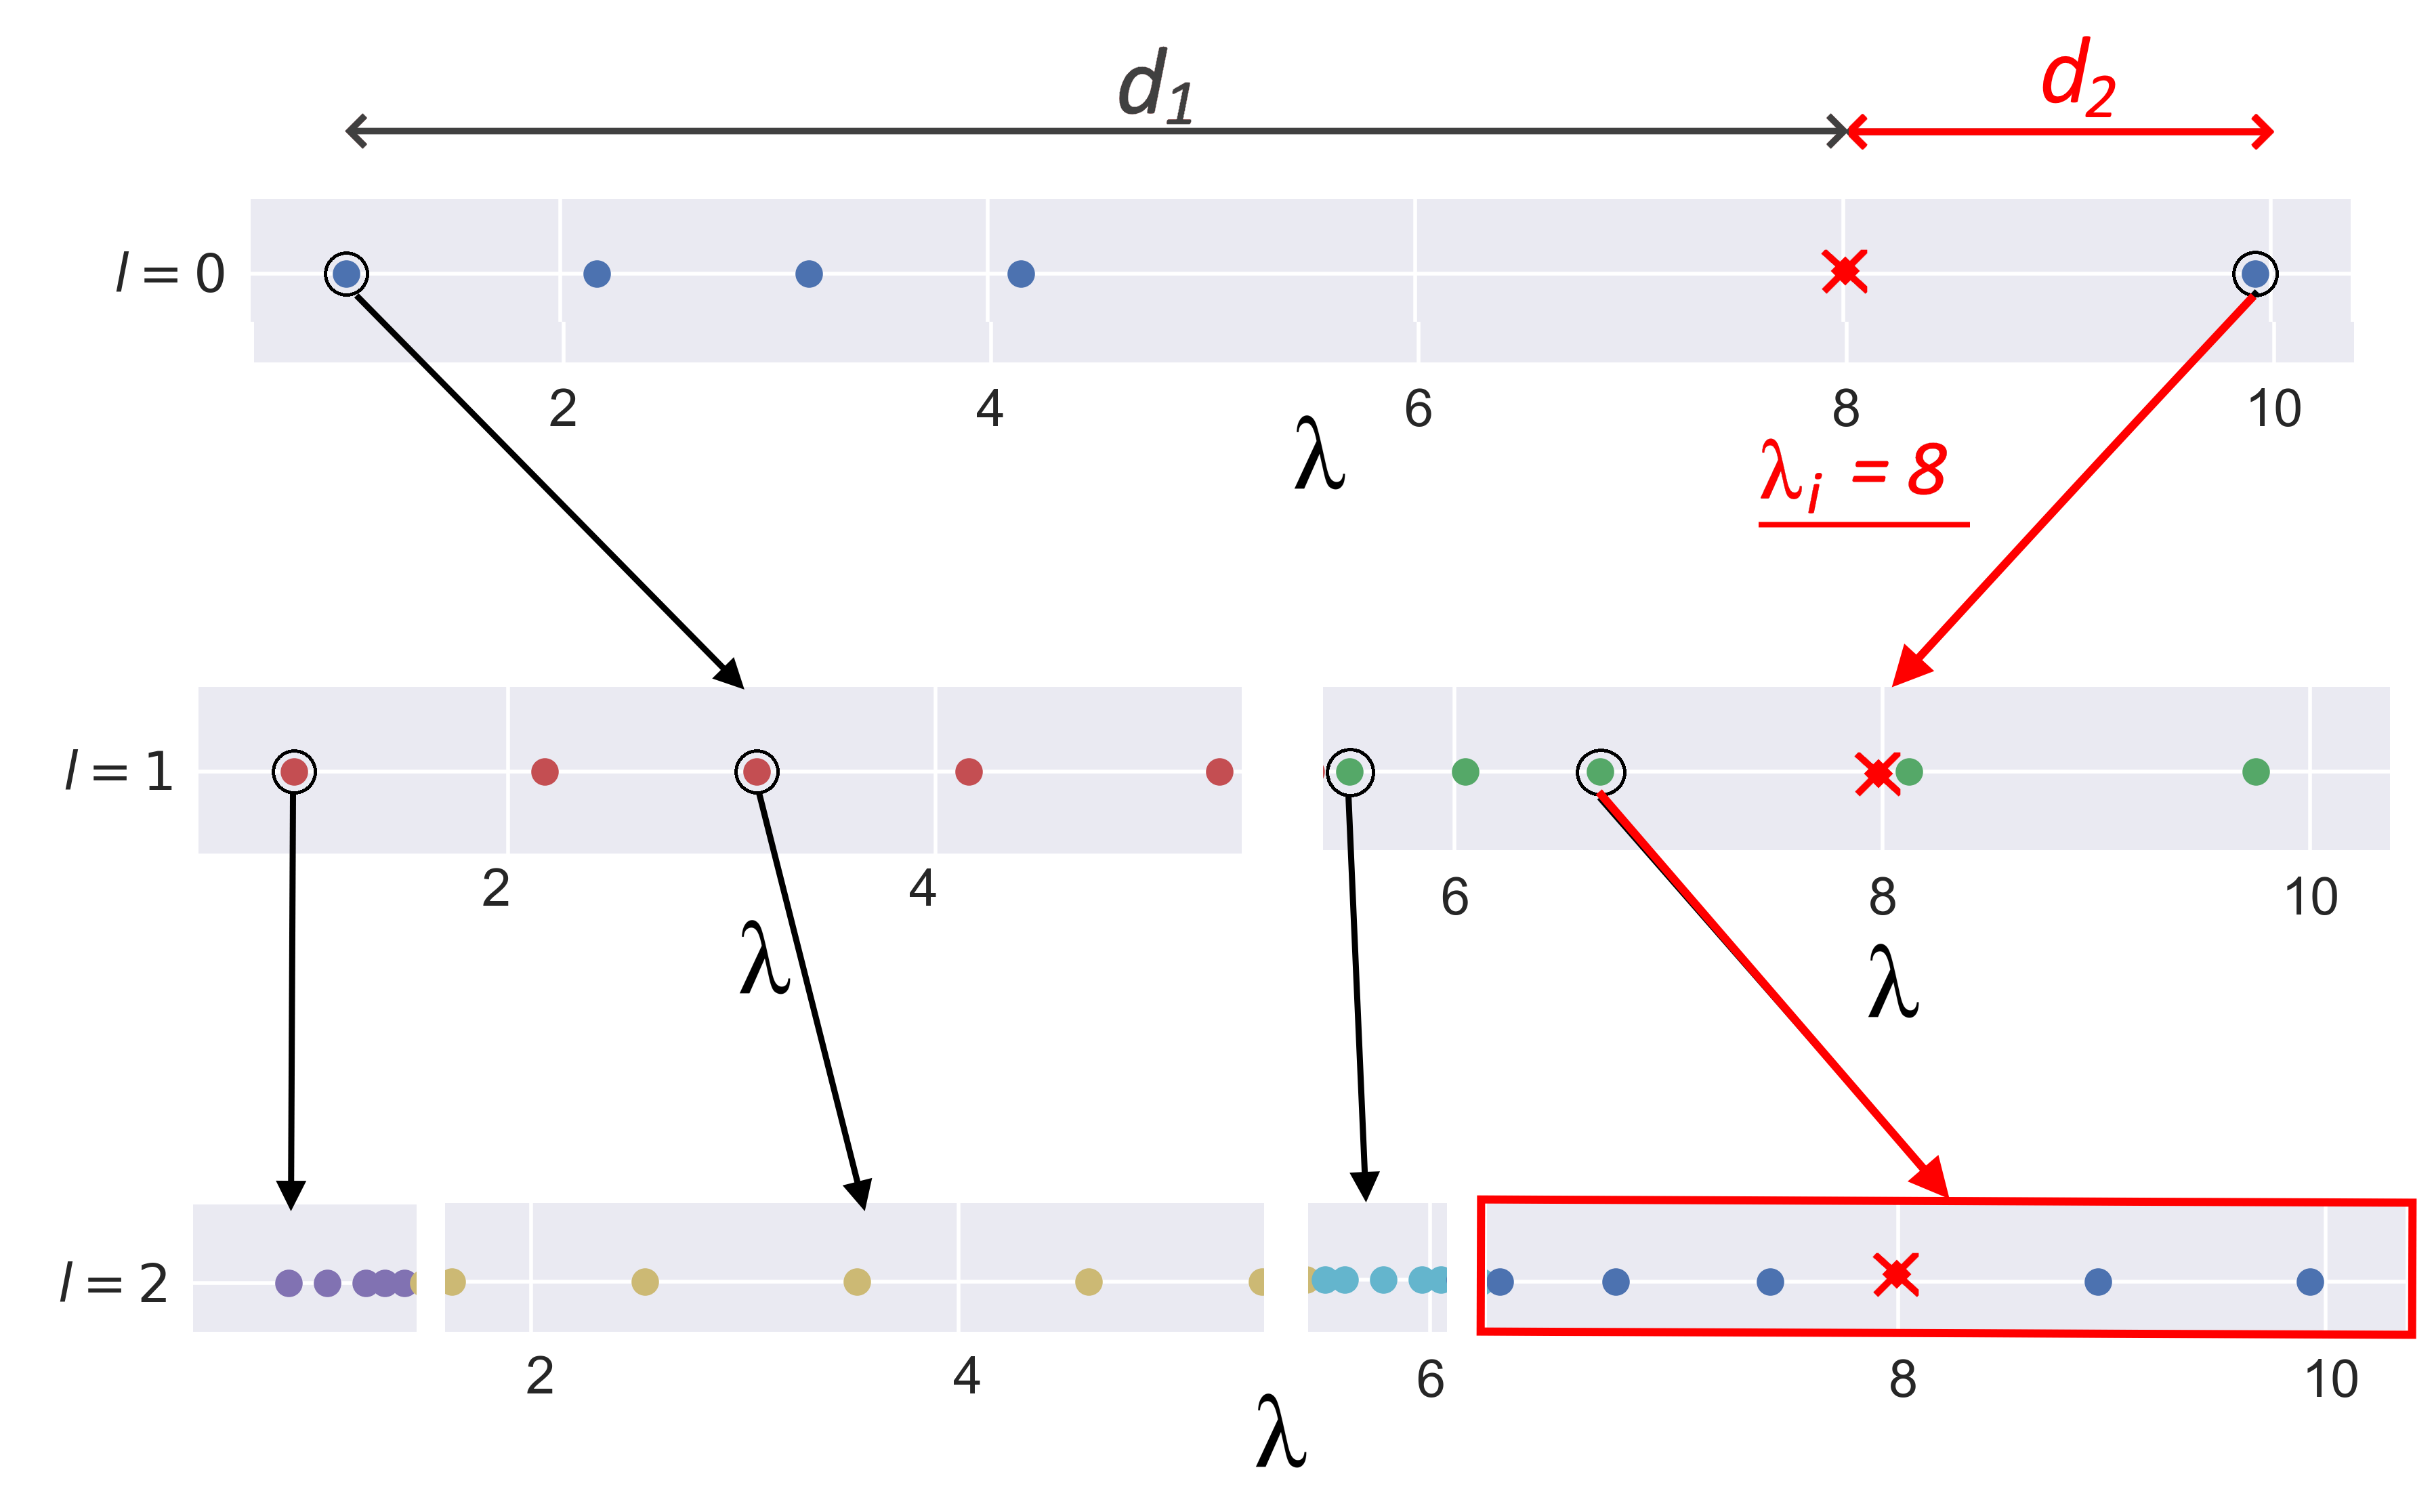
\includegraphics[width=0.75\columnwidth]{figs/proyeccion_1d.png}
\caption{Proyección de una onda $h_{\lambda_i}$ sobre la base de ejemplo de la figura \ref{fig:part_1d} (en este caso $\lambda_i = 8$, marcado con una cruz roja). Partiendo de la raíz del árbol, se calcula iterativamente la distancia entre $\lambda_i$ y los puntos de anclaje de cada subdominio, hasta llegar a alguna de las hojas del árbol.}
\label{fig:proy_1d}
\end{figure}

Al momento de proyectar una función $h_{\lambda_i}$ a una base \textit{hp-greedy}, primero se debe obtener la base local del nodo hoja (ver fig. \ref{fig:proy_1d}) y luego se realiza la proyección a la base encontrada.
Proyectar un conjunto de validación implica repetir este mismo proceso para todas las funciones del conjunto. Este proceso se realizará a lo largo de un tiempo $t$, que se denomina \textit{tiempo de proyección}. 

En el siguiente apartado se analiza el tiempo de proyección en diferentes bases \textit{hp-greedy} en el contexto de ondas gravitacionales.


\subsection{Aplicación a Ondas Gravitacionales}
\label{sec:hp-gw}

En esta subsección se utiliza un conjunto de ondas gravitacionales con parámetro bidimensional $\lambda = (q, \chi_z)$, donde $\chi_{1_z} = \chi_{2_z} = \chi_z$ es el espín de los agujeros negros y $q$ es la relación entre sus masas. De esta forma se puede graficar fácilmente el dominio de parámetros.



En la figura \ref{fig:part1} se puede observar una representación de la partición del dominio de parámetros. En la primera imagen se pueden ver los dos puntos de anclaje, que son los primeros dos elementos de la base global construida inicialmente. En cada nueva división se construye una nueva base global con la cual se realiza la siguiente partición de cada subdominio.


\begin{figure}[h!]
\centering
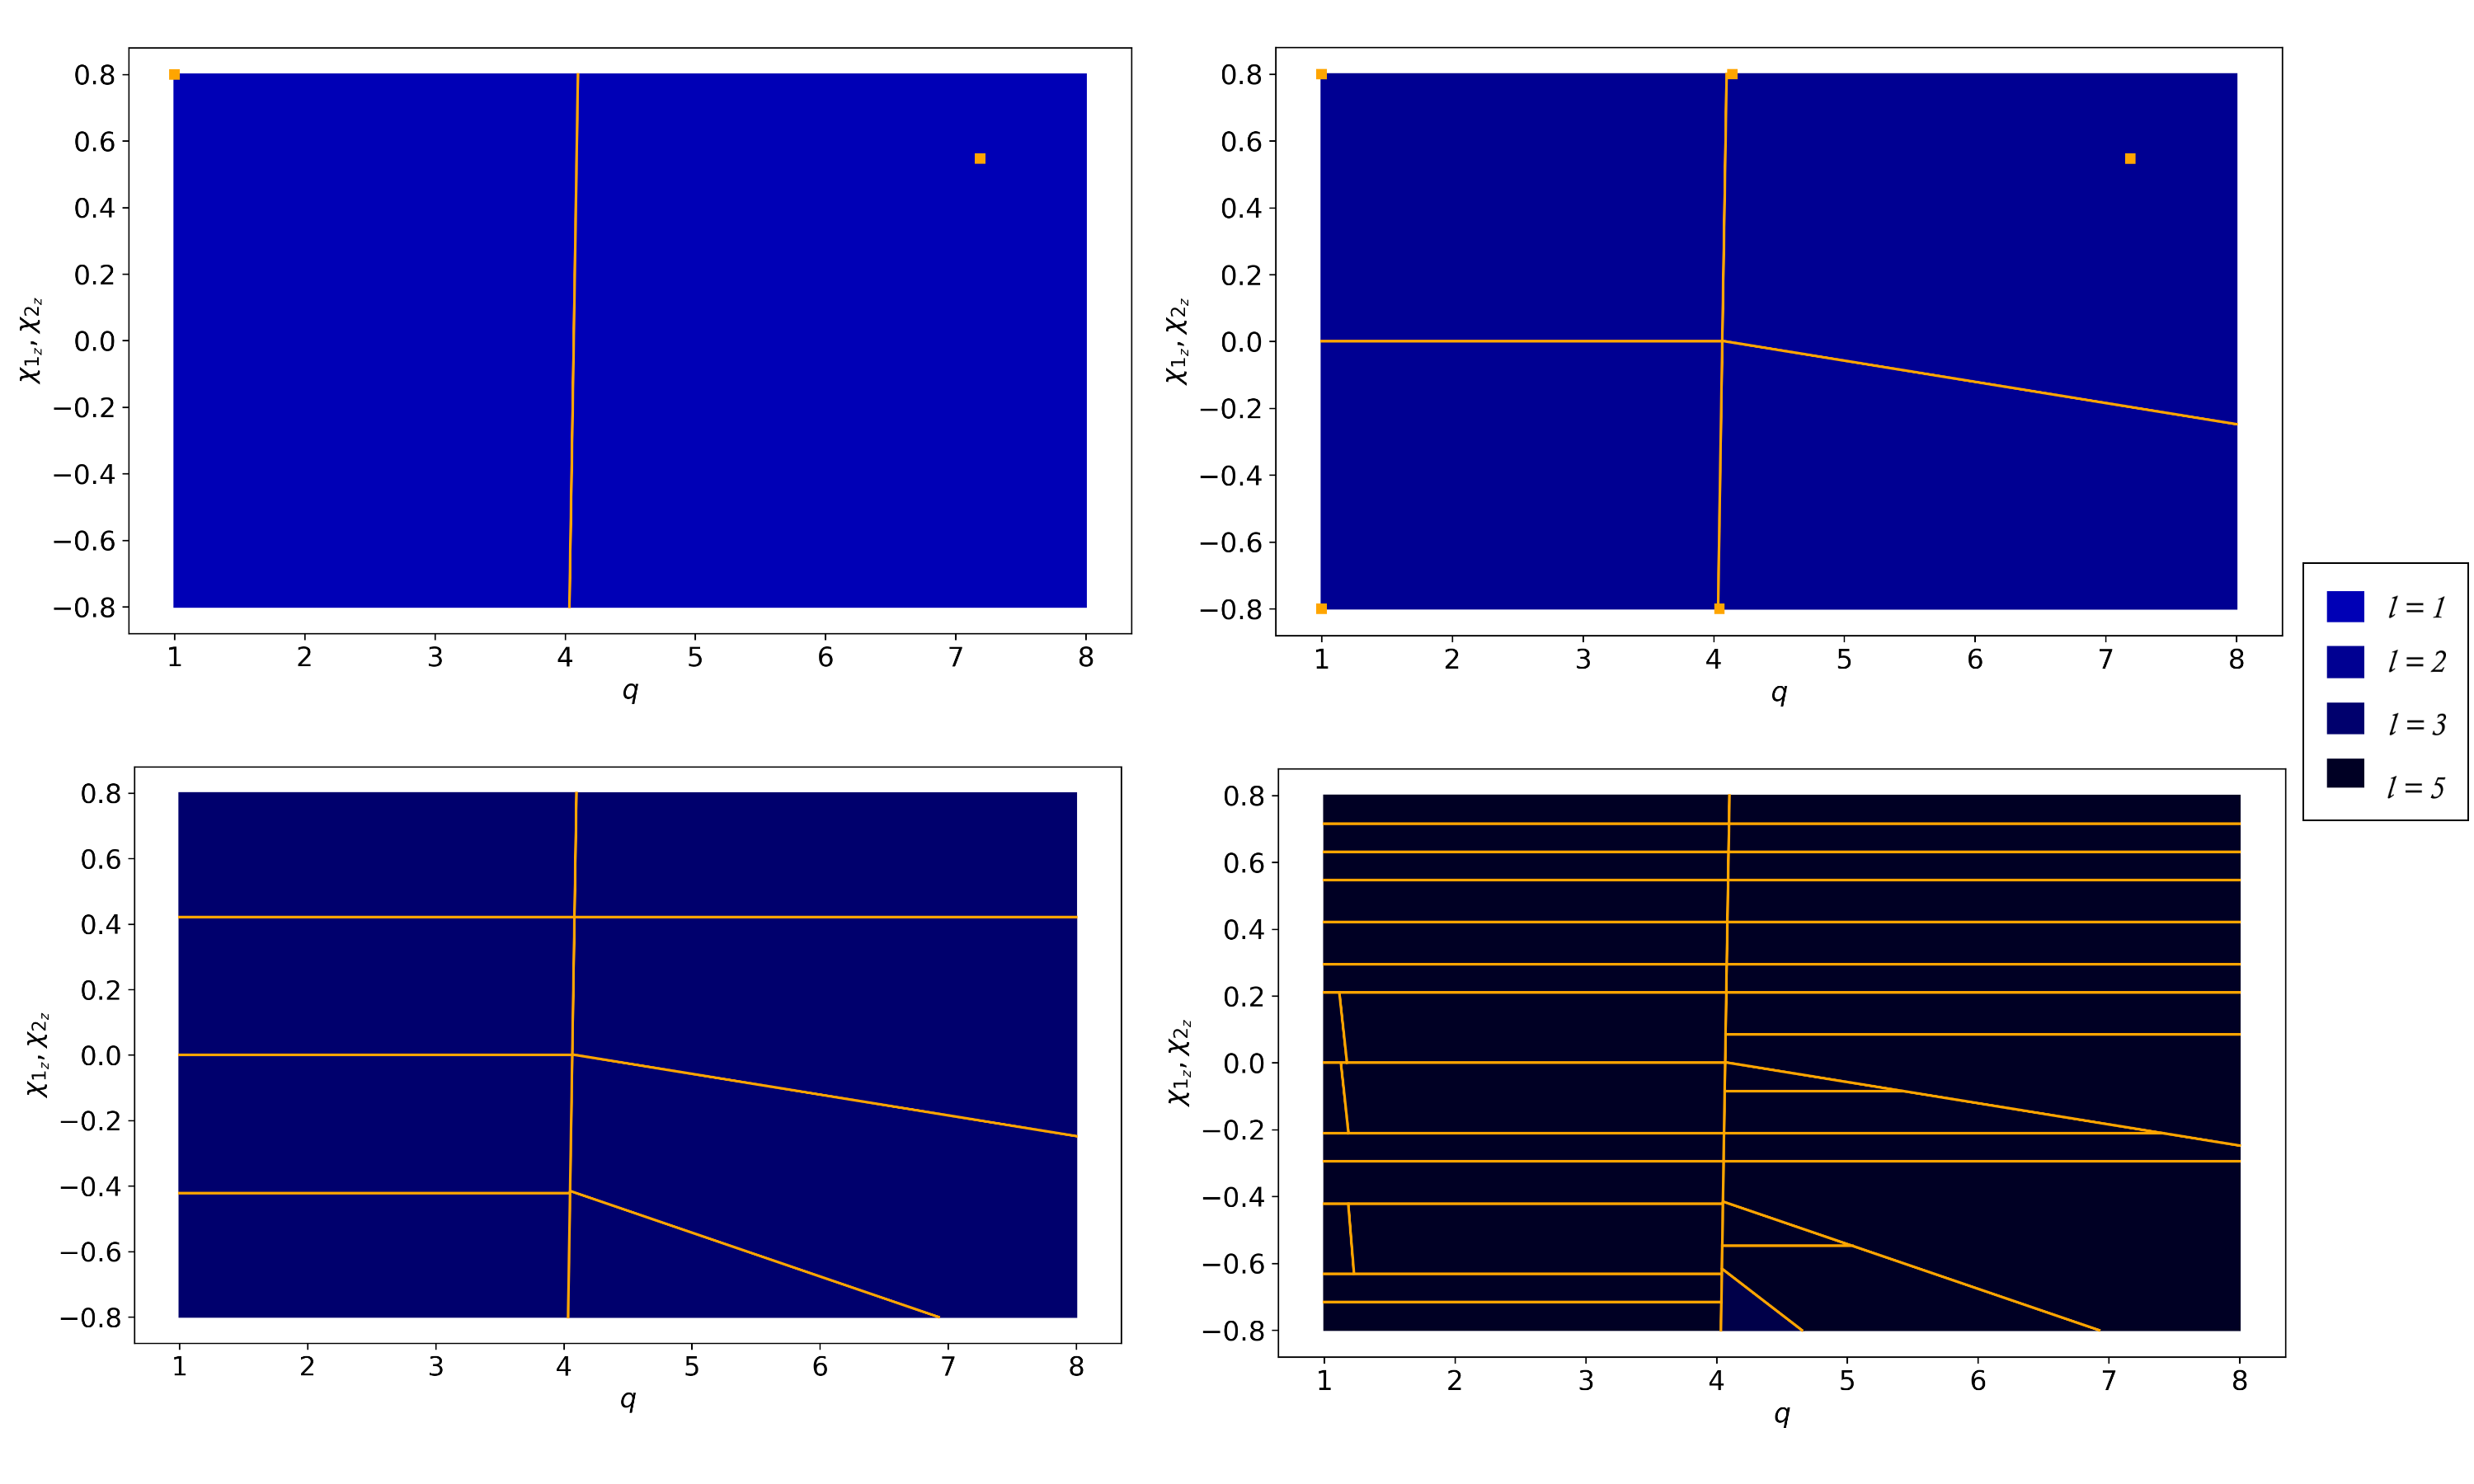
\includegraphics[width=1\columnwidth]{figs/particion2d.png}
\caption{Ejemplo de partición del espacio de parámetros bidimensional para $l_{max}= 1, 2, 3$ y $5$. En los primeros dos casos se muestran los puntos de anclaje en naranja.}
\label{fig:part1}
\end{figure}


En la figure \ref{fig:l0vl4} se compara el máximo error de representación obtenido para un conjunto de validación con una base global, es decir, con $l_{max} = 0$, y con $l_{max}=4$. La velocidad de convergencia es claramente mayor en el segundo caso.

\begin{figure}[h!]
\centering
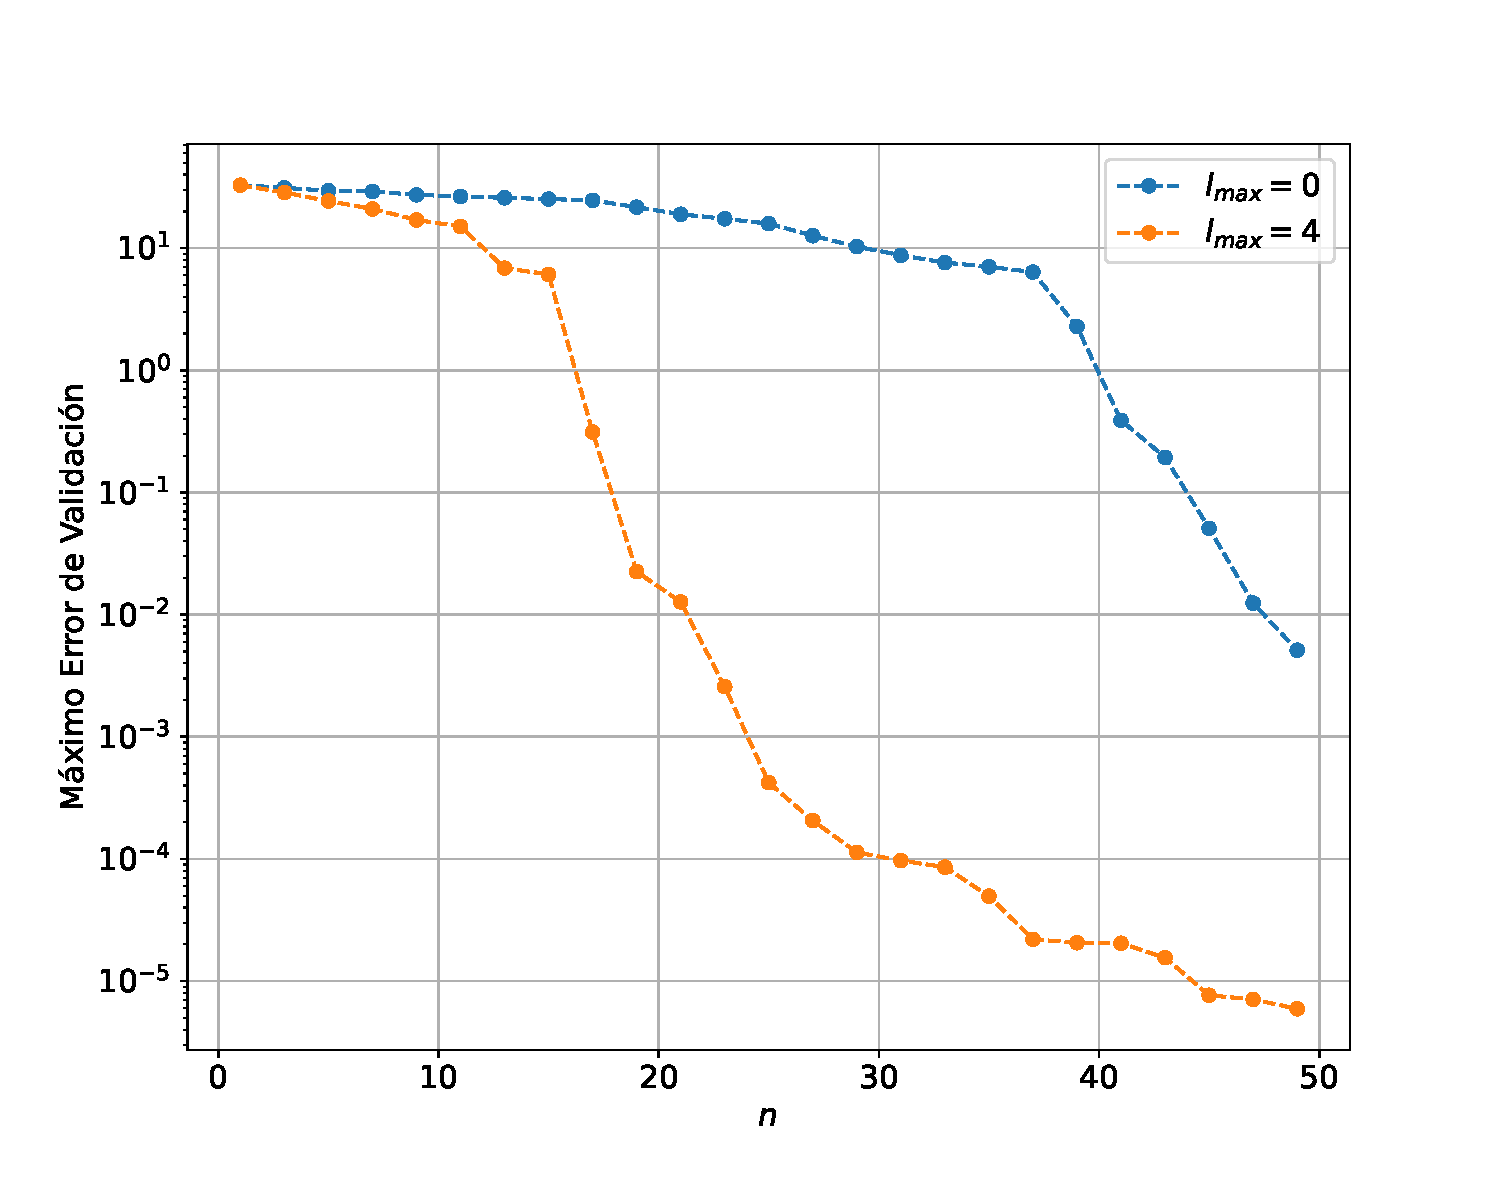
\includegraphics[width=.8\columnwidth, trim={0, 1.3cm, 0, 1.4cm}]{figs/l0vsl4.pdf}
\caption{Base global ($l_{max} = 0$) versus base con $l_{max} = 4$} para distintos valores de $n$.
\label{fig:l0vl4}
\end{figure}



\begin{figure}[h!]
\centering
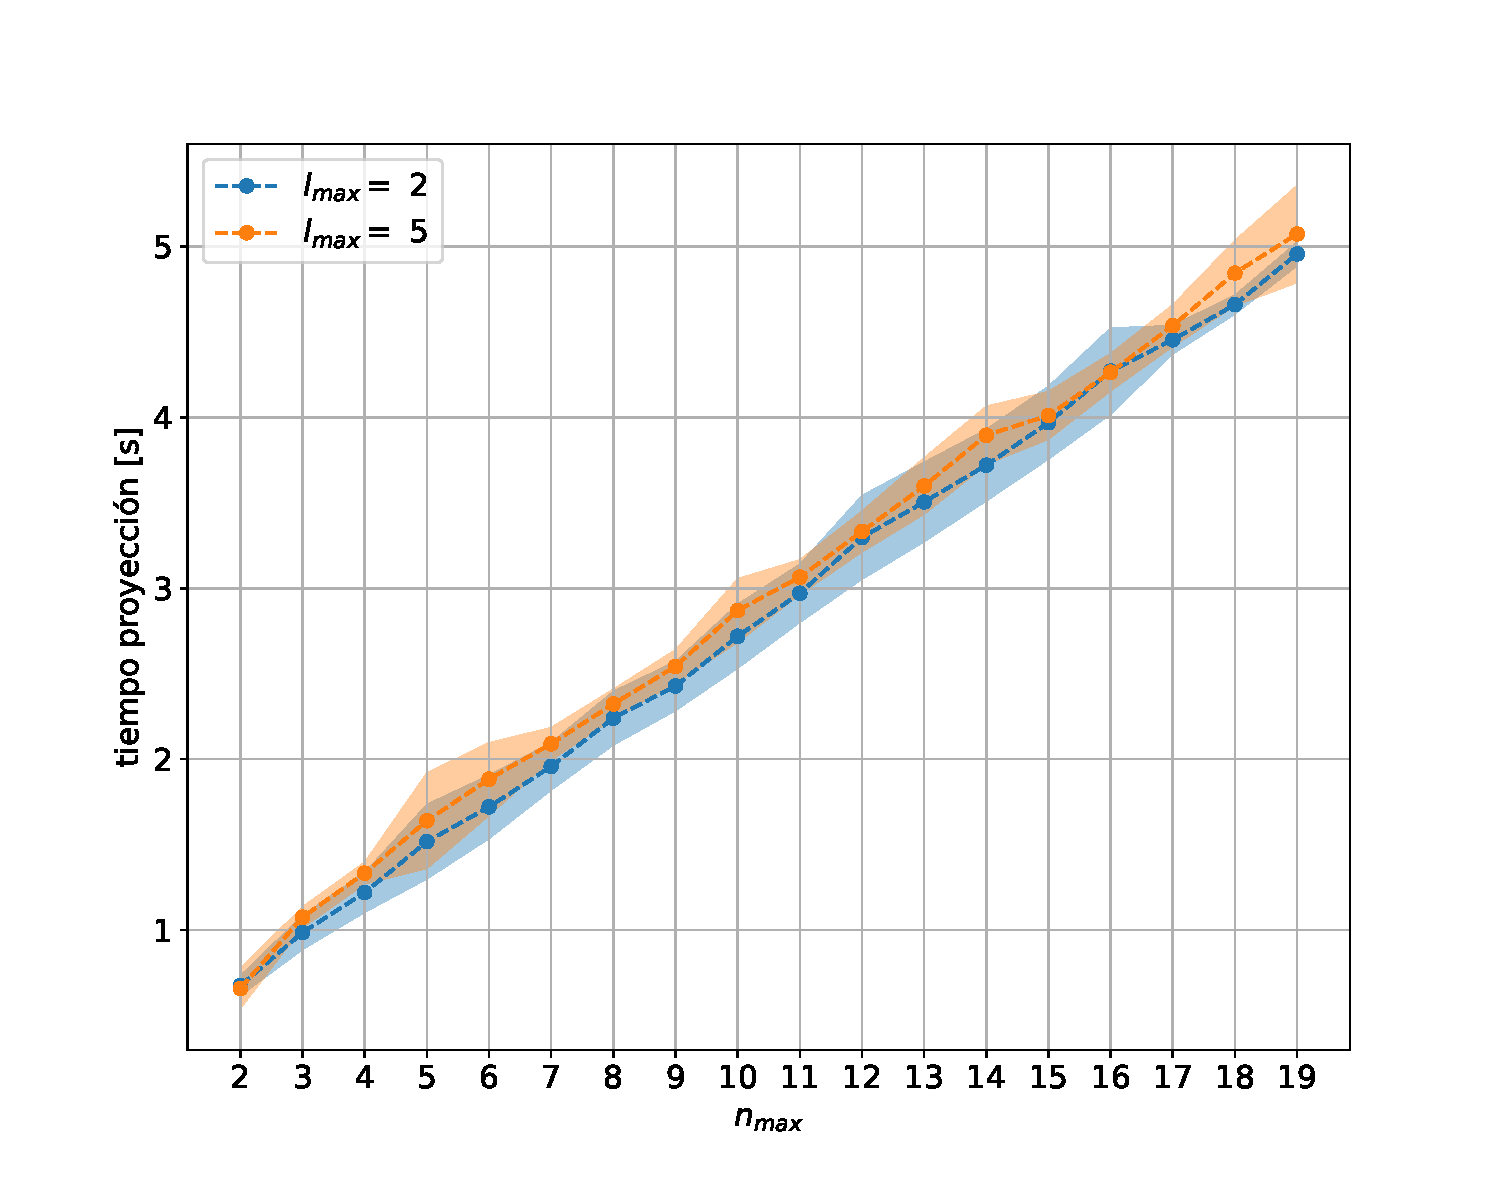
\includegraphics[width=.8\columnwidth ,trim={0, 1cm, 0, 1.2cm}]{figs/t_vs_nmax.pdf}
\caption{tiempos de proyección de un conjunto de validación a dos bases con distinto $l_{max}$ en función del $n_{max}$. En cada caso la linea de trazo representa el valor medio, y el área de color indica una desviación estandar desde el valor medio, para cada medición.}
\label{fig:t_vs_nmax}
\end{figure}


En la figura \ref{fig:t_vs_nmax} se graficó el tiempo de proyección de un conjunto de validación a dos bases \textit{hp-greedy} con distinto valor de $l_{max}$. Se observa que el tiempo es bastante lineal en relación al $n$ (elementos de las bases locales), y no parece ser afectado por $l_{max}$.



\begin{figure}[h!]
\centering
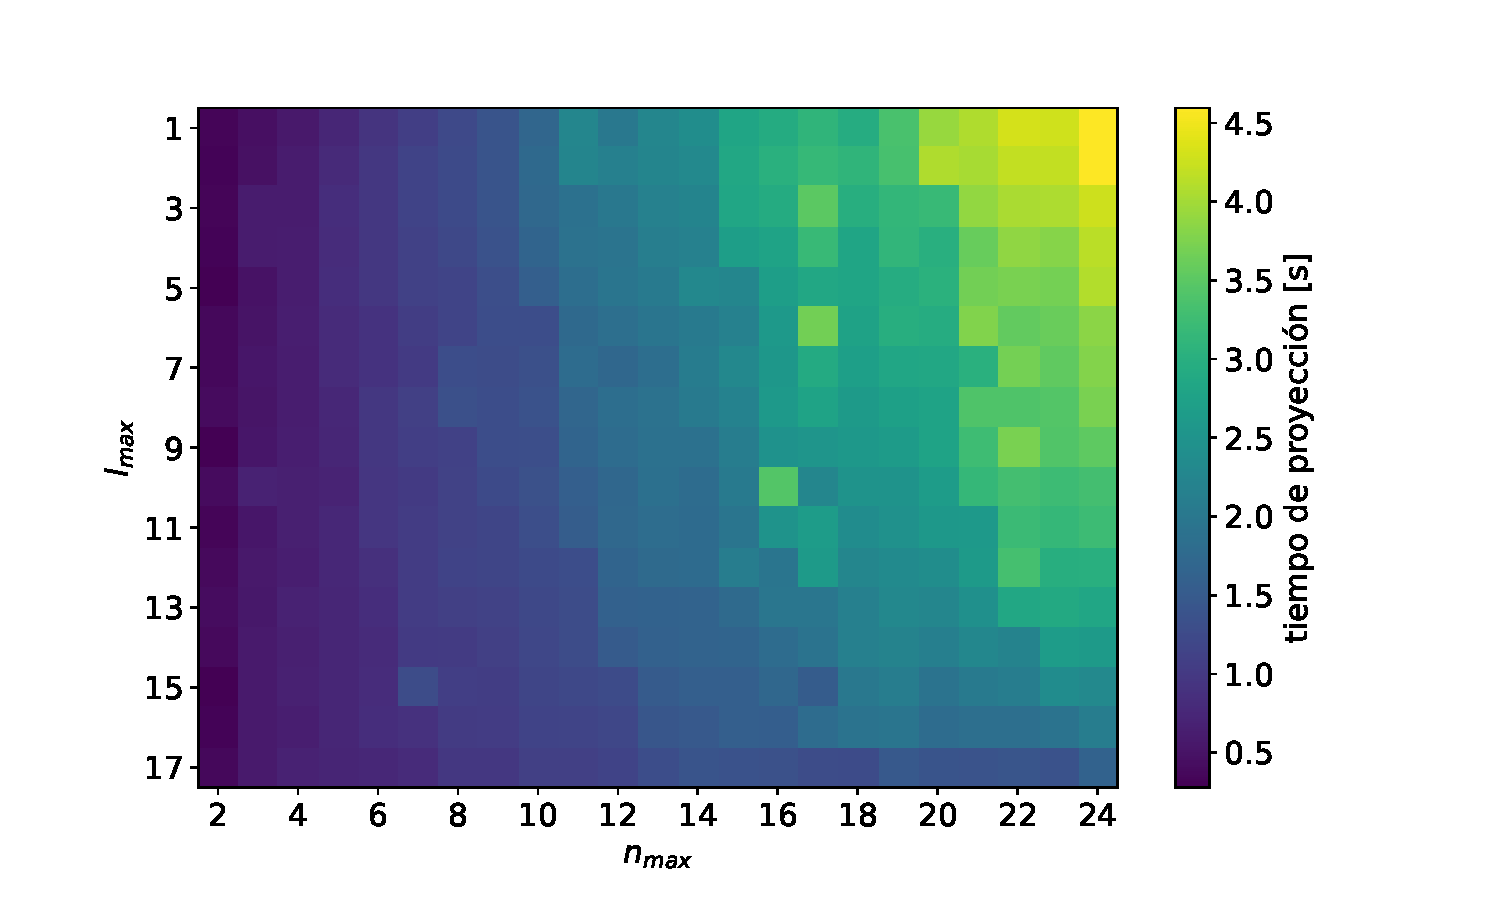
\includegraphics[width=.9\columnwidth, trim={0, 1cm, 0, 1.4cm}]{figs/nmax_lmax_t_grid.pdf}
\caption{Tiempo de proyección de un conjunto de validación para diferentes valores de $n_{max}$ y $l_{max}$}
\label{fig:t_grilla_nl}
\end{figure}


En la figura \ref{fig:t_grilla_nl} se puede ver el tiempo de proyección para más valores de $n_{max}$ y $l_{max}$. En los primeros valores de $l_{max}$ se observa un comportamiento similar al descrito anteriormente, donde el tiempo depende casi únicamente de $n_{max}$. Sin embargo al aumentar el $l_{max}$ se observa que el tiempo disminuye. Esto se puede entender en dos partes:

\begin{itemize}
\item \textbf{Independencia aparente entre el tiempo de proyección y $l_{max}$}: para realizar la proyección de cada onda del conjunto de validación en la base \textit{hp-greedy} primero se debe buscar el subdominio (la hoja) correspondiente utilizando los puntos de anclaje de la estructura arbórea de la base. Luego se proyectará la onda en la base local del subdominio en cuestión. Si bien la búsqueda en el árbol tiene una complejidad temporal $O(l_{max})$, el trabajo de cómputo más importante es el que se realizará al momento de proyectar la base, que es independiente de $l_{max}$, con una complejidad temporal $O(n_{max})$. Pero esto solo se cumple hasta ciertos valores de $l_{max}$.
\item \textbf{Disminución del tiempo de proyección al aumentar $l_{max}$}: ya se mencionó en más de una ocasión que por cada nivel $l$ hay un máximo de $2^l$ subdominios. Es decir que si se quiere obtener el número de elementos de todas las bases en las hojas del árbol, suponiendo un árbol denso, este número será $n_{max} \times 2^{l_{max}}$. En la figura \ref{fig:t_grilla_nl} se utilizó un conjunto de entrenamiento con 1400 ondas, por lo que al llegar a unos valores de $l_{max} = 6$ y $n_{max} = 24$ en total debería haber 1536 elementos de base en total. Es decir, más elementos de base que ondas en el conjunto de entrenamiento. Por lo tanto al aumentar el $l_{max}$ rápidamente se aumenta el número de subdominios, reduciendo su tamaño como resultado y reduciendo el número de elementos de las bases locales (cada subdominio tendrá una cantidad de elementos menor a $n_{max}$). De esta forma se explica la disminución del tiempo de proyección para valores grandes de $l_{max}$, consecuencia del tamaño limitado del conjunto de entrenamiento.
\end{itemize}


\subsection{Hiperparámetros}

\begin{figure}[h!]
\centering
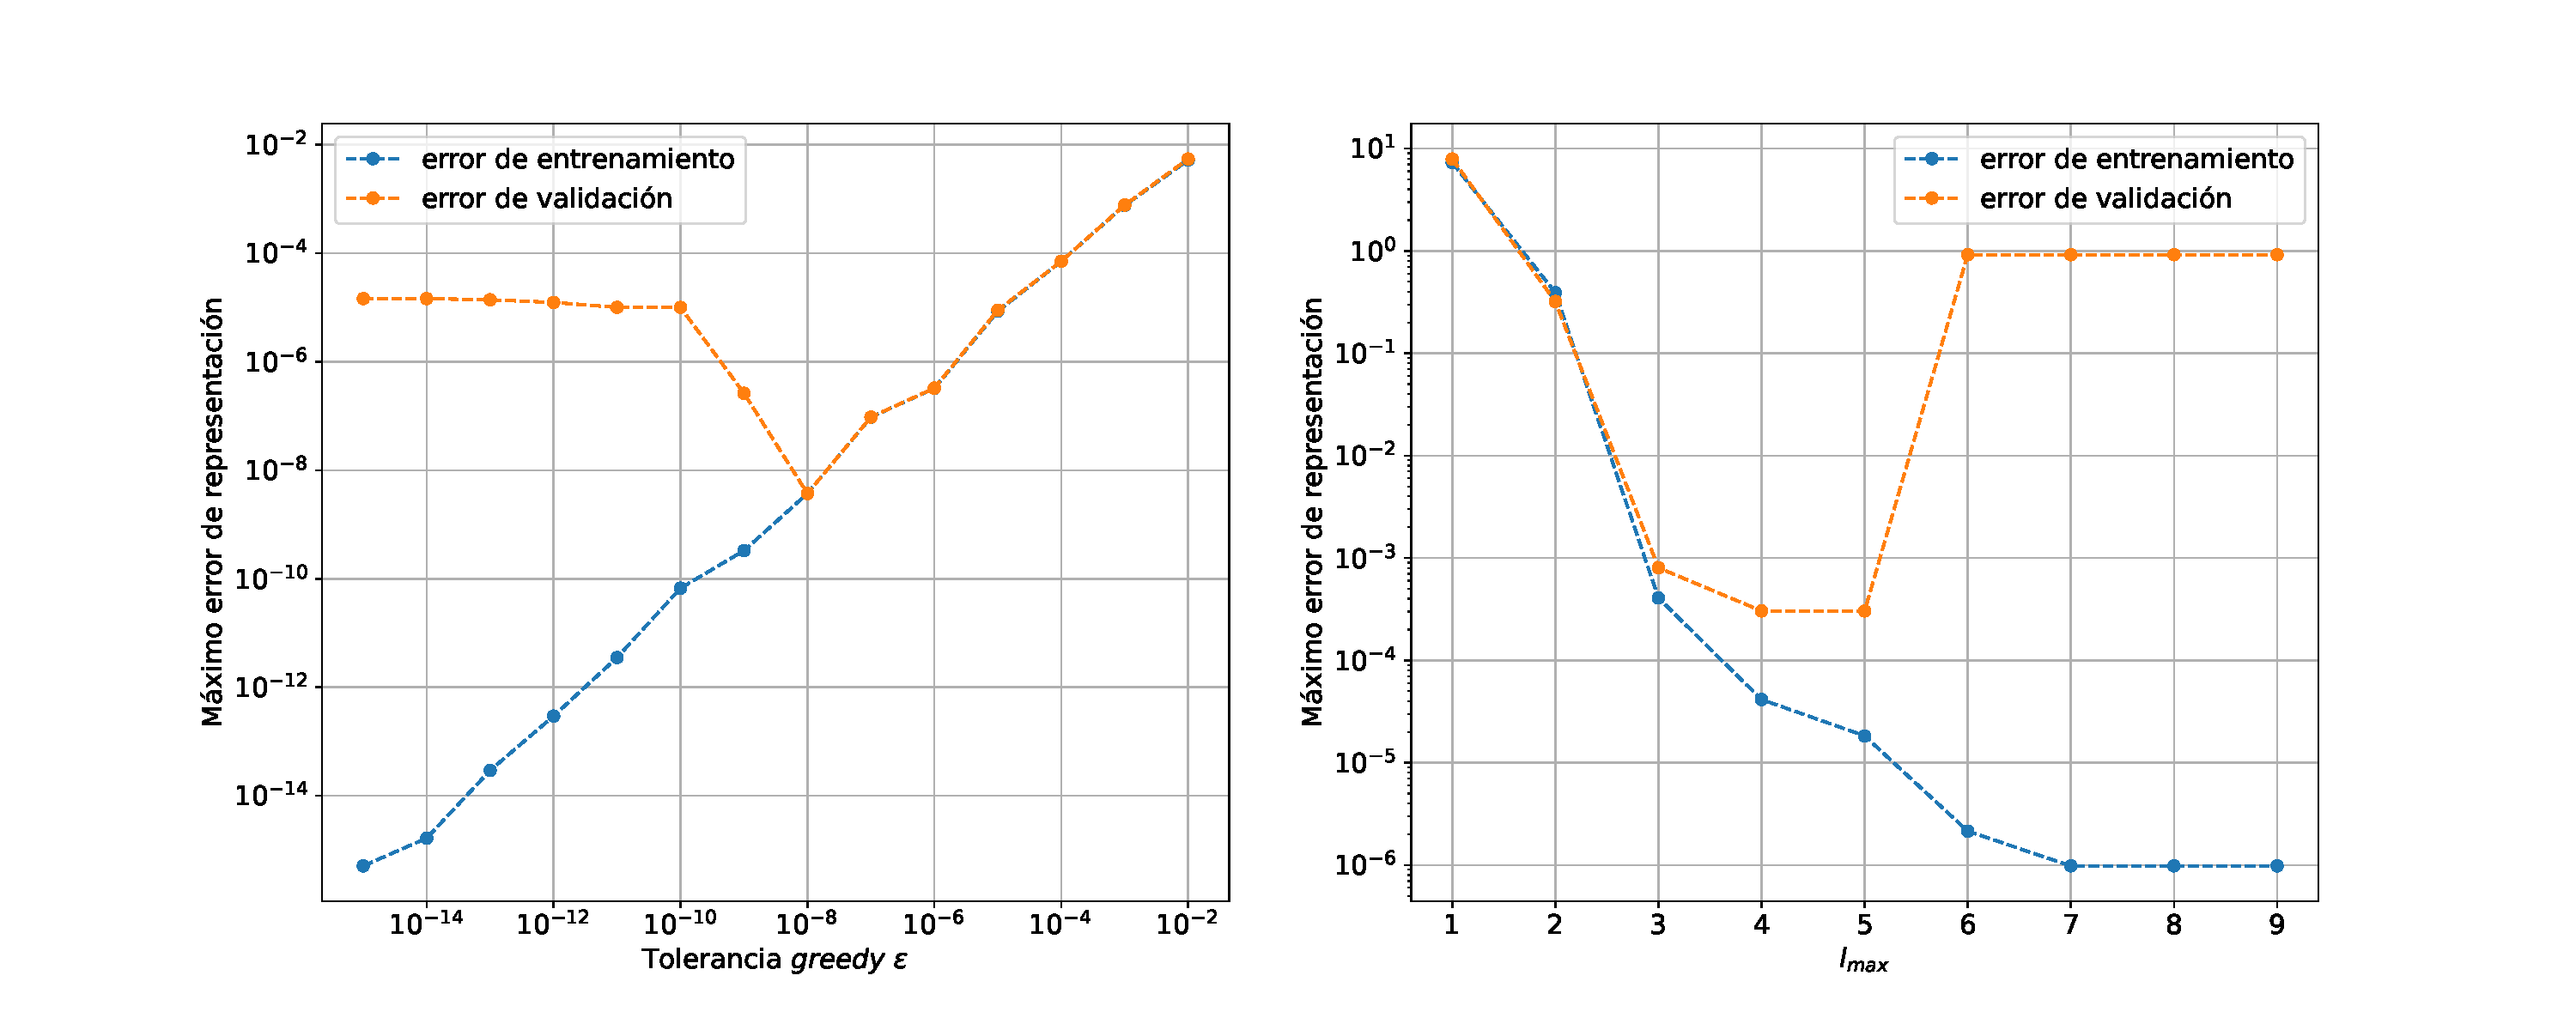
\includegraphics[width=1\columnwidth ,trim={2cm, 1cm, 1cm, 1.2cm}]{figs/overfit.pdf}
\caption{Ejemplos de \textit{sobreajuste}. A la izquierda variando $\varepsilon$ con $(n_{max}, l_{max}) = (25, 19)$ en un conjunto de parámetro unidimensional $(\lambda_i = q_i)$. A la derecha variando $l_{max}$ con $(n_{max}, \varepsilon) = (20, 1\times10^{-6})$ en un conjunto de parámetro bidimensional$(\lambda_{ij} = (q_i, \chi_{z_j})) $.}
\label{fig:overfit}
\end{figure}

Al momento de construir una base \textit{hp-greedy} entran en juego cuatro hiperparámetros. Los primeros tres son los parámetros de parada;
\begin{itemize}
\item $\bm{n_{max}}:$ determina la cantidad máxima de elementos para cada base local. A mayor cantidad de elementos el error de representación será menor, pero el tiempo requerido para proyectar un conjunto de validación a la base depende casi exclusivamente de este hiperparámetro.
\item $\bm{l_{max}}:$ determina la máxima profundidad de las hojas del árbol. En general al aumentar $l_{max}$ disminuye el error de representación, pero valores muy elevados junto a cierta combinación de hiperparámetros pueden dar lugar a sobreajustes en el modelo, un ejemplo de esto se puede ver en la figura \ref{fig:overfit}. Este es un comportamiento típico de las estructuras arbóreas.
\item $\bm{\varepsilon}$: la tolerancia \textit{greedy} interviene tanto en el tamaño de las bases locales como en la profundidad de las hojas del árbol. Un valor de $\varepsilon$ demasiado bajo también puede dar lugar a sobreajuste, sobre todo con valores muy altos de $l_{max}$. Un valor de $\varepsilon = 0$ implica que se obtiene un árbol totalmente denso, determinado únicamente por $n_{max}$ y $l_{max}$, y al aumentar el valor de $\varepsilon$ se puede pensar en la analogía de podar un árbol, de forma que se previene el sobreajuste.
\end{itemize}

Al cuarto hiperparámetro se le da el nombre de \textit{\textbf{semilla}} y en este trabajo se la denota con $\bm{\hat{\Lambda}_0}$ para diferenciarla de la semilla de una base local, denotada por $\Lambda_1$;

\begin{figure}[h!]
\centering
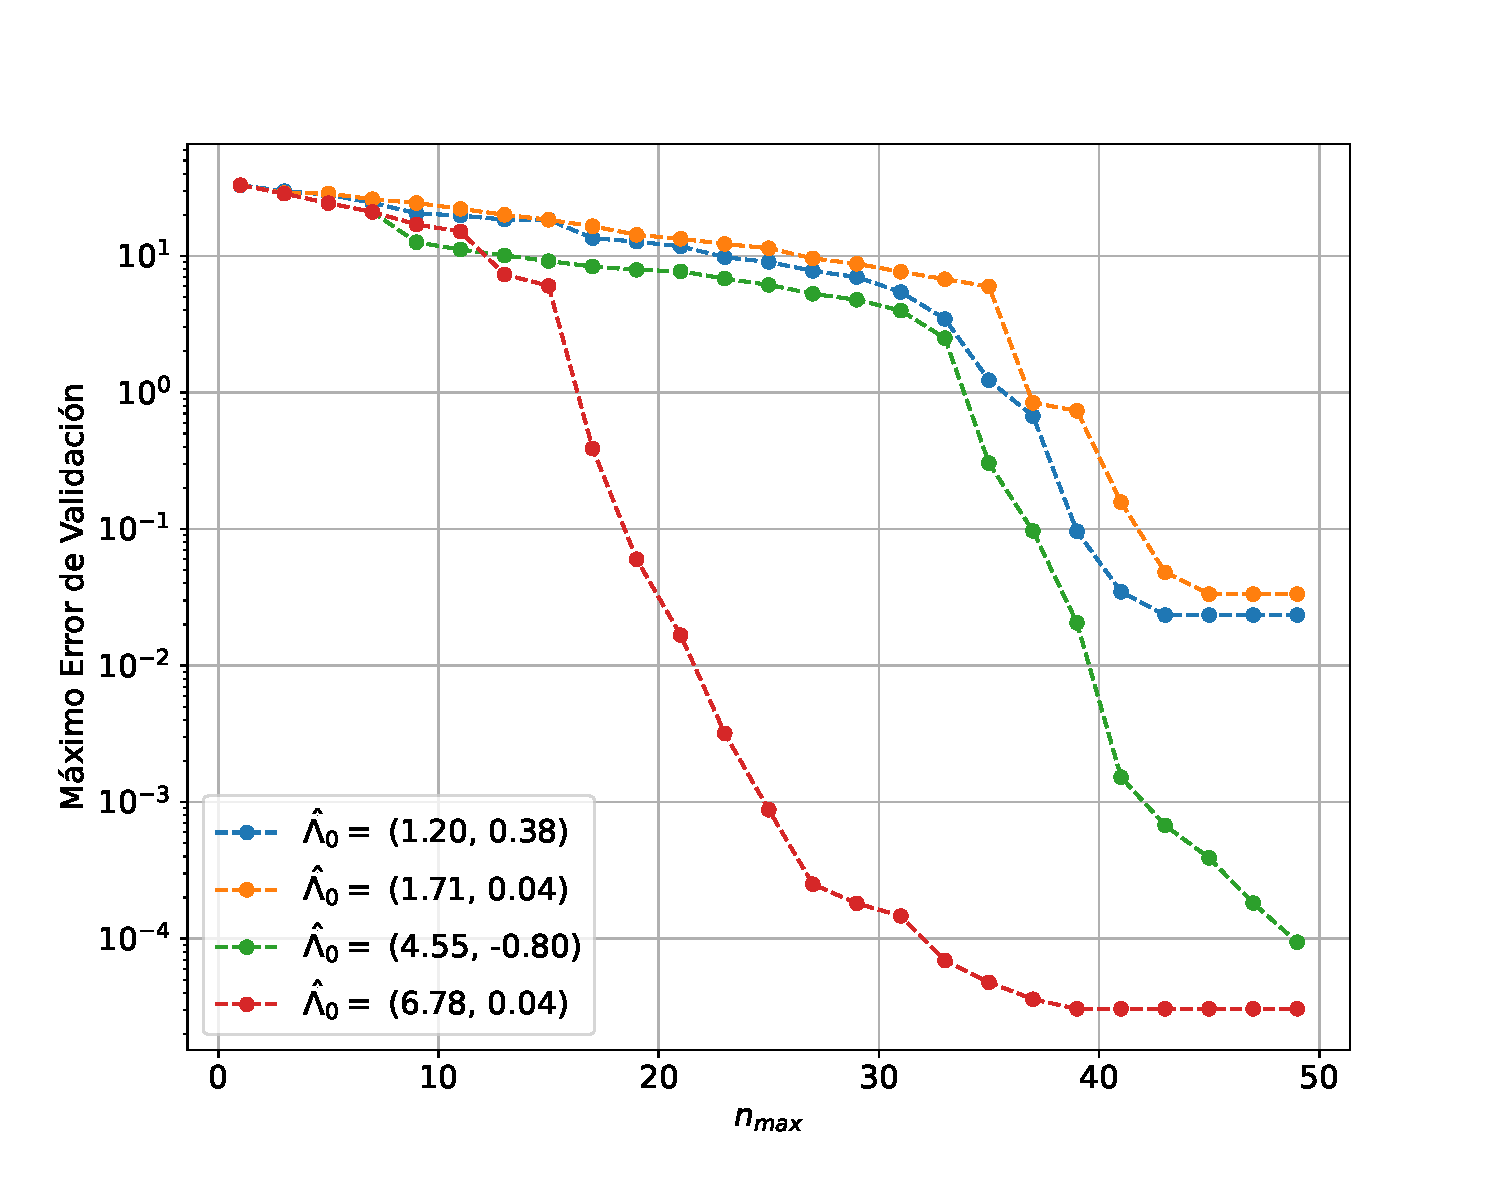
\includegraphics[width=.8\columnwidth ,trim={1.1cm, 1.1cm, 1.2cm, 1.2cm}]{figs/Semillas_v_nmax_2D.pdf}
\caption{Error de validación para diferentes semillas.}
\label{fig:seeds0}
\end{figure}

\begin{itemize}
\item $\bm{\hat{\Lambda}_0}$: la semilla no es más que el primer parámetro \textit{greedy} de la base global. En cada base local, el primer parámetro \textit{greedy} no es relevante, pero en el caso de las bases \textit{hp-greedy} cada semilla dará lugar a una división diferente del dominio de parámetros. En la figura \ref{fig:seeds0} se puede ver como cuatro semillas diferentes dan lugar a cuatro curvas de error con distinta convergencia. En la figura \ref{fig:seeds_part}, por otro lado, se observa el resultado de la partición del dominio para tres semillas diferentes. En general las semillas que mejor funcionan (con el conjunto de datos utilizado) son las que logran una partición regular del dominio de parámetros.
\end{itemize}

\begin{figure}[h!]
\centering
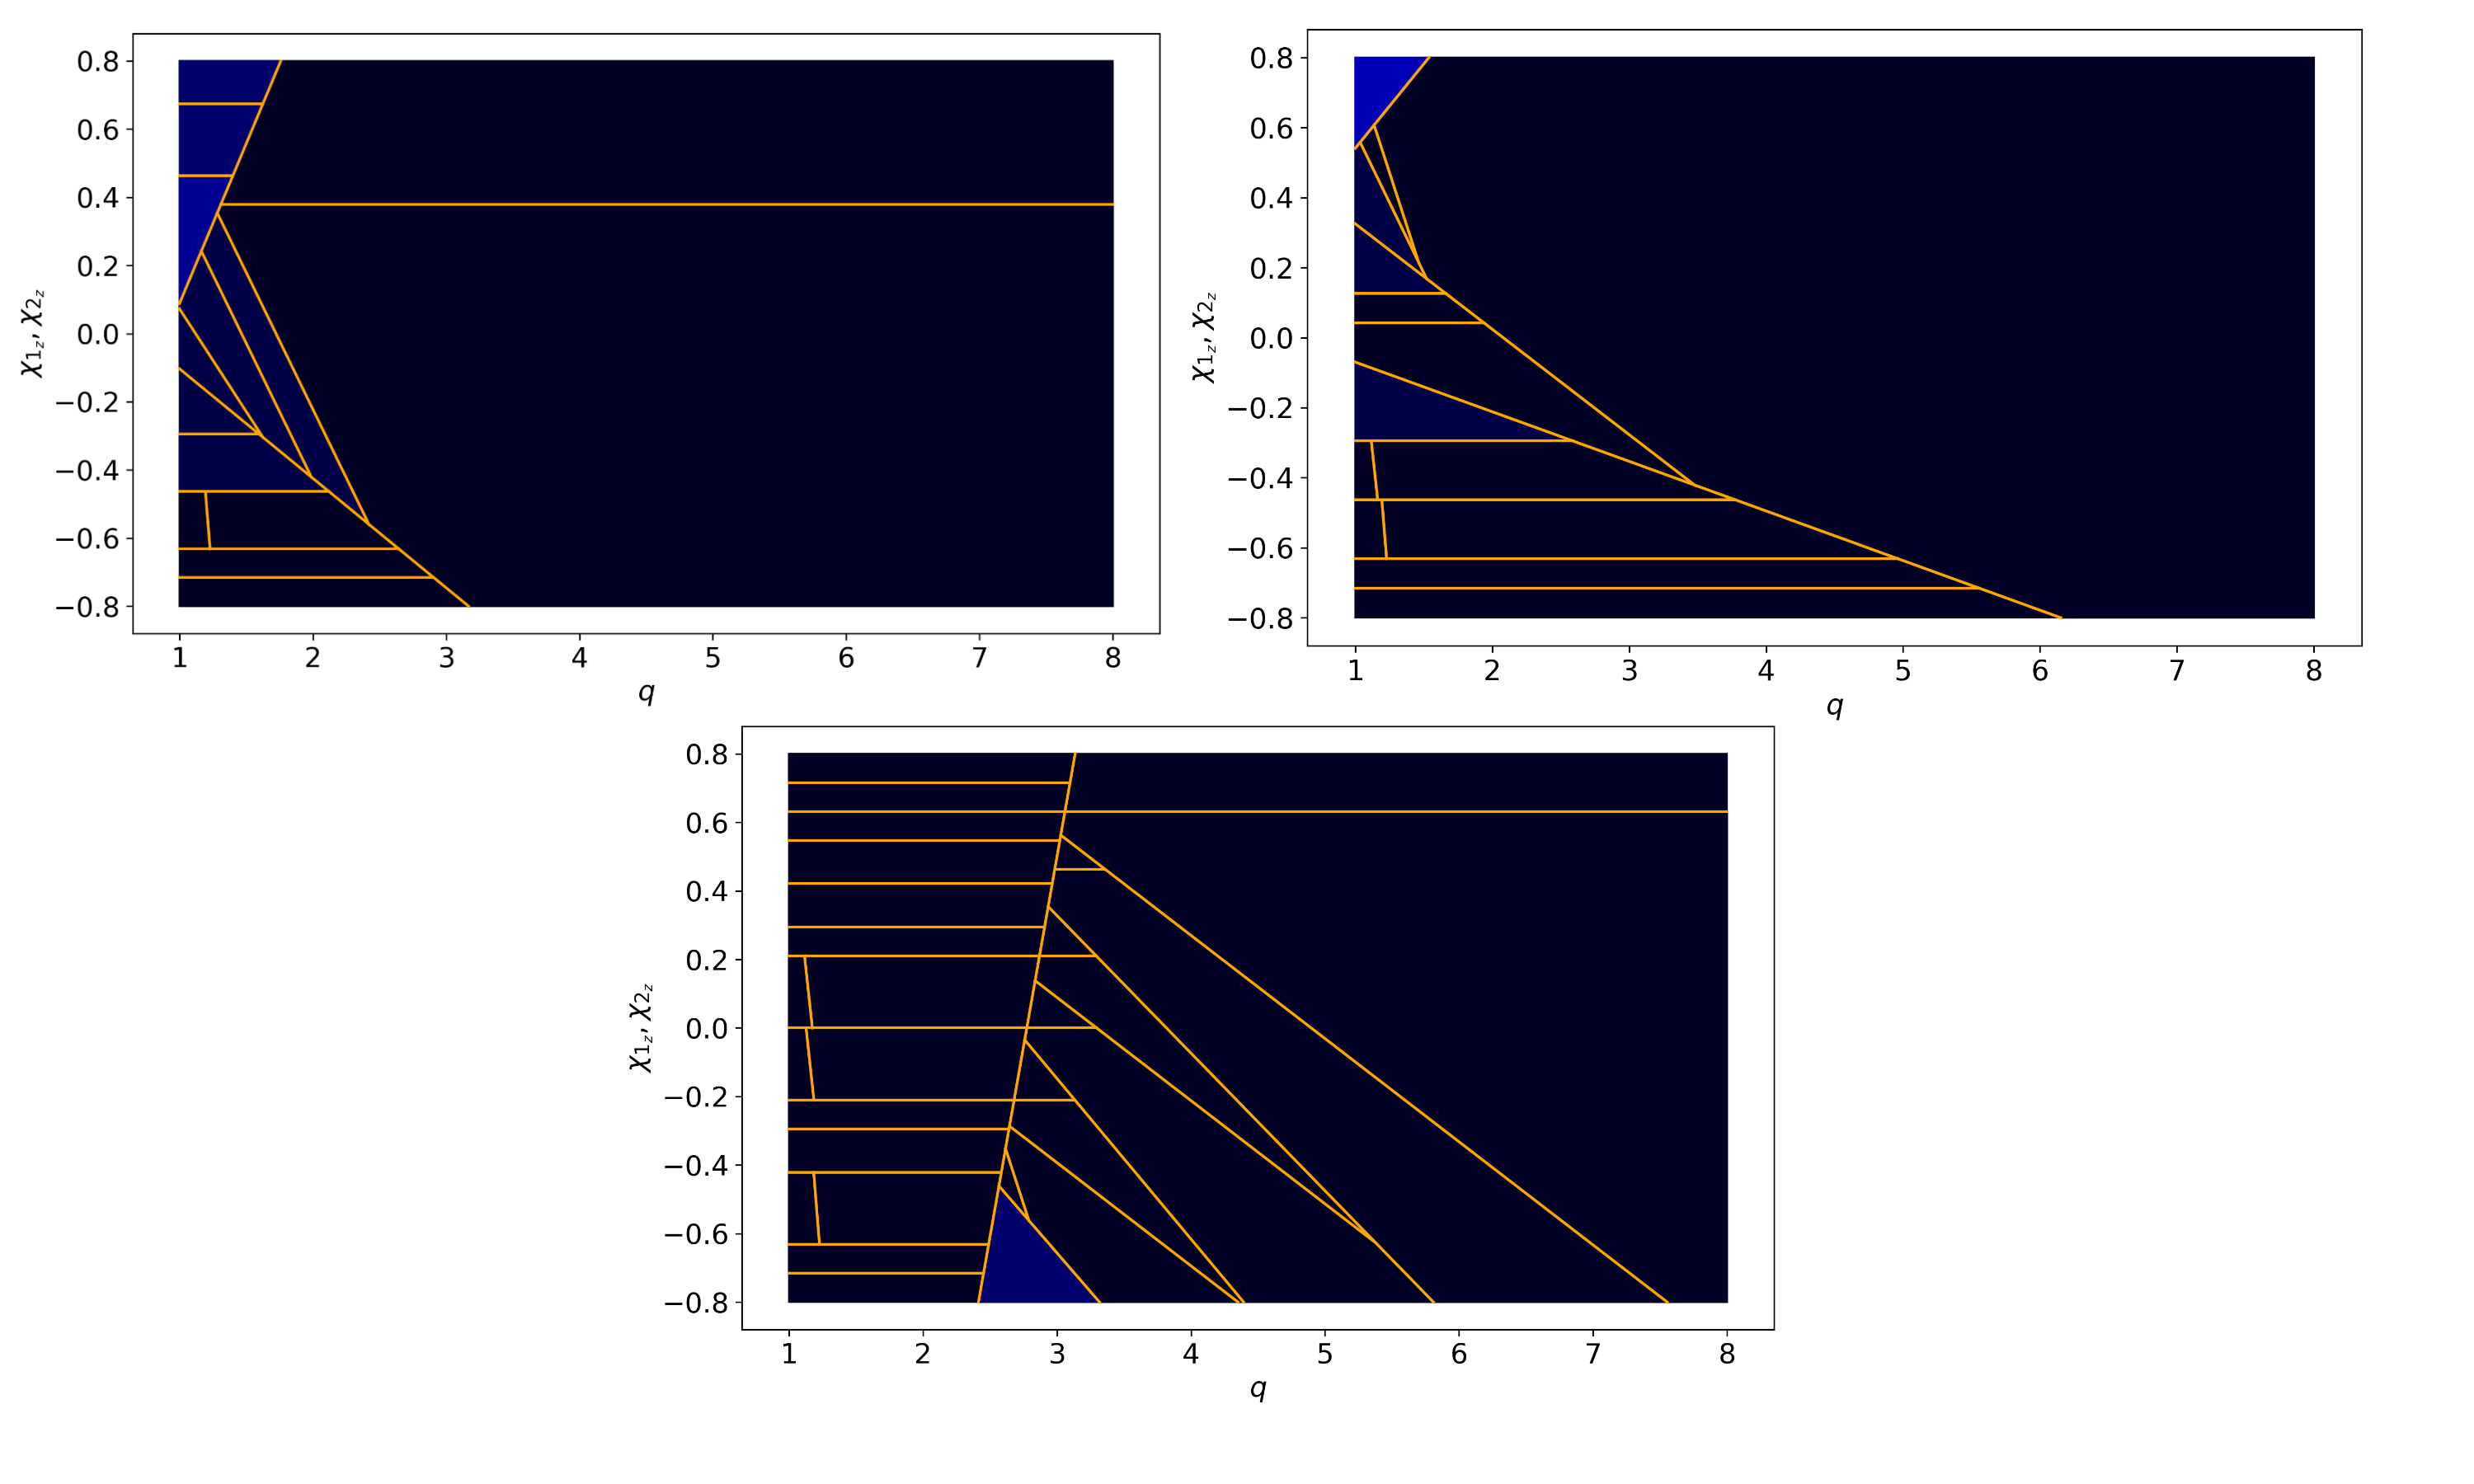
\includegraphics[width=1.05\columnwidth ,trim={1.1cm, 1cm, 1cm, 1.2cm}]{figs/3_semillas_particion.png}
\caption{Partición del espacio de parámetros para tres semillas diferentes; a la izquierda $\hat{\Lambda}_0 = (1.2 \ \ 0.38)$, a la derecha $\hat{\Lambda}_0 = (1.71 \ \ 0.04)$ y al centro $\hat{\Lambda}_0 =(4.55 \ \ -0.8)$.}
\label{fig:seeds_part}
\end{figure}